% Options for packages loaded elsewhere
\PassOptionsToPackage{unicode}{hyperref}
\PassOptionsToPackage{hyphens}{url}
\PassOptionsToPackage{dvipsnames,svgnames,x11names}{xcolor}
%
\documentclass[
  ignorenonframetext,
  aspectratio=169]{beamer}
\usepackage{pgfpages}
\setbeamertemplate{caption}[numbered]
\setbeamertemplate{caption label separator}{: }
\setbeamercolor{caption name}{fg=normal text.fg}
\beamertemplatenavigationsymbolsempty
% Prevent slide breaks in the middle of a paragraph
\widowpenalties 1 10000
\raggedbottom
\setbeamertemplate{part page}{
  \centering
  \begin{beamercolorbox}[sep=16pt,center]{part title}
    \usebeamerfont{part title}\insertpart\par
  \end{beamercolorbox}
}
\setbeamertemplate{section page}{
  \centering
  \begin{beamercolorbox}[sep=12pt,center]{part title}
    \usebeamerfont{section title}\insertsection\par
  \end{beamercolorbox}
}
\setbeamertemplate{subsection page}{
  \centering
  \begin{beamercolorbox}[sep=8pt,center]{part title}
    \usebeamerfont{subsection title}\insertsubsection\par
  \end{beamercolorbox}
}
\AtBeginPart{
  \frame{\partpage}
}
\AtBeginSection{
  \ifbibliography
  \else
    \frame{\sectionpage}
  \fi
}
\AtBeginSubsection{
  \frame{\subsectionpage}
}
\usepackage{amsmath,amssymb}
\usepackage{lmodern}
\usepackage{iftex}
\ifPDFTeX
  \usepackage[T1]{fontenc}
  \usepackage[utf8]{inputenc}
  \usepackage{textcomp} % provide euro and other symbols
\else % if luatex or xetex
  \usepackage{unicode-math}
  \defaultfontfeatures{Scale=MatchLowercase}
  \defaultfontfeatures[\rmfamily]{Ligatures=TeX,Scale=1}
\fi
\usetheme[]{CambridgeUS}
% Use upquote if available, for straight quotes in verbatim environments
\IfFileExists{upquote.sty}{\usepackage{upquote}}{}
\IfFileExists{microtype.sty}{% use microtype if available
  \usepackage[]{microtype}
  \UseMicrotypeSet[protrusion]{basicmath} % disable protrusion for tt fonts
}{}
\makeatletter
\@ifundefined{KOMAClassName}{% if non-KOMA class
  \IfFileExists{parskip.sty}{%
    \usepackage{parskip}
  }{% else
    \setlength{\parindent}{0pt}
    \setlength{\parskip}{6pt plus 2pt minus 1pt}}
}{% if KOMA class
  \KOMAoptions{parskip=half}}
\makeatother
\usepackage{xcolor}
\newif\ifbibliography
\usepackage{color}
\usepackage{fancyvrb}
\newcommand{\VerbBar}{|}
\newcommand{\VERB}{\Verb[commandchars=\\\{\}]}
\DefineVerbatimEnvironment{Highlighting}{Verbatim}{commandchars=\\\{\}}
% Add ',fontsize=\small' for more characters per line
\usepackage{framed}
\definecolor{shadecolor}{RGB}{248,248,248}
\newenvironment{Shaded}{\begin{snugshade}}{\end{snugshade}}
\newcommand{\AlertTok}[1]{\textcolor[rgb]{0.94,0.16,0.16}{#1}}
\newcommand{\AnnotationTok}[1]{\textcolor[rgb]{0.56,0.35,0.01}{\textbf{\textit{#1}}}}
\newcommand{\AttributeTok}[1]{\textcolor[rgb]{0.77,0.63,0.00}{#1}}
\newcommand{\BaseNTok}[1]{\textcolor[rgb]{0.00,0.00,0.81}{#1}}
\newcommand{\BuiltInTok}[1]{#1}
\newcommand{\CharTok}[1]{\textcolor[rgb]{0.31,0.60,0.02}{#1}}
\newcommand{\CommentTok}[1]{\textcolor[rgb]{0.56,0.35,0.01}{\textit{#1}}}
\newcommand{\CommentVarTok}[1]{\textcolor[rgb]{0.56,0.35,0.01}{\textbf{\textit{#1}}}}
\newcommand{\ConstantTok}[1]{\textcolor[rgb]{0.00,0.00,0.00}{#1}}
\newcommand{\ControlFlowTok}[1]{\textcolor[rgb]{0.13,0.29,0.53}{\textbf{#1}}}
\newcommand{\DataTypeTok}[1]{\textcolor[rgb]{0.13,0.29,0.53}{#1}}
\newcommand{\DecValTok}[1]{\textcolor[rgb]{0.00,0.00,0.81}{#1}}
\newcommand{\DocumentationTok}[1]{\textcolor[rgb]{0.56,0.35,0.01}{\textbf{\textit{#1}}}}
\newcommand{\ErrorTok}[1]{\textcolor[rgb]{0.64,0.00,0.00}{\textbf{#1}}}
\newcommand{\ExtensionTok}[1]{#1}
\newcommand{\FloatTok}[1]{\textcolor[rgb]{0.00,0.00,0.81}{#1}}
\newcommand{\FunctionTok}[1]{\textcolor[rgb]{0.00,0.00,0.00}{#1}}
\newcommand{\ImportTok}[1]{#1}
\newcommand{\InformationTok}[1]{\textcolor[rgb]{0.56,0.35,0.01}{\textbf{\textit{#1}}}}
\newcommand{\KeywordTok}[1]{\textcolor[rgb]{0.13,0.29,0.53}{\textbf{#1}}}
\newcommand{\NormalTok}[1]{#1}
\newcommand{\OperatorTok}[1]{\textcolor[rgb]{0.81,0.36,0.00}{\textbf{#1}}}
\newcommand{\OtherTok}[1]{\textcolor[rgb]{0.56,0.35,0.01}{#1}}
\newcommand{\PreprocessorTok}[1]{\textcolor[rgb]{0.56,0.35,0.01}{\textit{#1}}}
\newcommand{\RegionMarkerTok}[1]{#1}
\newcommand{\SpecialCharTok}[1]{\textcolor[rgb]{0.00,0.00,0.00}{#1}}
\newcommand{\SpecialStringTok}[1]{\textcolor[rgb]{0.31,0.60,0.02}{#1}}
\newcommand{\StringTok}[1]{\textcolor[rgb]{0.31,0.60,0.02}{#1}}
\newcommand{\VariableTok}[1]{\textcolor[rgb]{0.00,0.00,0.00}{#1}}
\newcommand{\VerbatimStringTok}[1]{\textcolor[rgb]{0.31,0.60,0.02}{#1}}
\newcommand{\WarningTok}[1]{\textcolor[rgb]{0.56,0.35,0.01}{\textbf{\textit{#1}}}}
\setlength{\emergencystretch}{3em} % prevent overfull lines
\providecommand{\tightlist}{%
  \setlength{\itemsep}{0pt}\setlength{\parskip}{0pt}}
\setcounter{secnumdepth}{-\maxdimen} % remove section numbering
\ifLuaTeX
\usepackage[bidi=basic]{babel}
\else
\usepackage[bidi=default]{babel}
\fi
\babelprovide[main,import]{spanish}
% get rid of language-specific shorthands (see #6817):
\let\LanguageShortHands\languageshorthands
\def\languageshorthands#1{}

%\usepackage[spanish,es-nolists]{babel}
%%\usepackage[spanish]{babel}
%% change fontsize of R code
%%colorines
\usepackage{amsmath,color,array,booktabs,algorithm2e}
%\newcommand\blue[1]{\textcolor{blue}{#1}}
%\newcommand\red[1]{\textcolor{red}{#1}}

%% change fontsize of output
\let\oldverbatim\verbatim
\let\endoldverbatim\endverbatim
\renewenvironment{verbatim}{\tiny\oldverbatim}{\endoldverbatim}

%\usepackage[table,xcdraw]{xcolor}

\usepackage{makecell}
 \usepackage{booktabs}
 \usepackage{adjustbox}
 \usepackage{amsmath,color,array,booktabs,algorithm2e}
 \newcommand\blue[1]{\textcolor{blue}{#1}}
 \newcommand\red[1]{\textcolor{red}{#1}}
 \setbeamertemplate{navigation symbols}{}
 \setbeamertemplate{footline}[page number]
 \usepackage{mathdots}
\usepackage{yhmath}
\usepackage{mathdots}
\usepackage{MnSymbol}
\renewcommand{\contentsname}{Índice}
\renewcommand{\chaptername}{Parte}
\renewcommand{\sectionname}{Sección}
\ifLuaTeX
  \usepackage{selnolig}  % disable illegal ligatures
\fi
\IfFileExists{bookmark.sty}{\usepackage{bookmark}}{\usepackage{hyperref}}
\IfFileExists{xurl.sty}{\usepackage{xurl}}{} % add URL line breaks if available
\urlstyle{same} % disable monospaced font for URLs
\hypersetup{
  pdftitle={R básico},
  pdflang={es-ES},
  colorlinks=true,
  linkcolor={Maroon},
  filecolor={Maroon},
  citecolor={Blue},
  urlcolor={Blue},
  pdfcreator={LaTeX via pandoc}}

\title{R básico}
\author{}
\date{\vspace{-2.5em}10-2022}

\begin{document}
\frame{\titlepage}

\begin{frame}[allowframebreaks]
  \tableofcontents[hideallsubsections]
\end{frame}
\hypertarget{factores}{%
\section{Factores}\label{factores}}

\begin{frame}[fragile]{Factor}
\protect\hypertarget{factor}{}
\blue{Factor}: es como un vector, pero con una estructura interna más
rica que permite usarlo para clasificar observaciones

\begin{itemize}
\tightlist
\item
  \texttt{levels}: atributo del factor. Cada elemento del factor es
  igual a un nivel. Los niveles clasifican las entradas del factor. Se
  ordenan por orden alfabético
\item
  Para definir un factor, primero hemos de definir un vector y
  trasformarlo por medio de una de las funciones \texttt{factor()} o
  \texttt{as.factor()}.
\end{itemize}
\end{frame}

\begin{frame}[fragile]{La función factor()}
\protect\hypertarget{la-funciuxf3n-factor}{}
\begin{itemize}
\item
  \texttt{factor(vector,levels=...)}: define un factor a partir del
  vector y dispone de algunos parámetros que permiten modificar el
  factor que se crea:

  \begin{itemize}
  \tightlist
  \item
    \texttt{levels}: permite especificar los niveles e incluso añadir
    niveles que no aparecen en el vector
  \item
    \texttt{labels}: permite cambiar los nombres de los niveles
  \end{itemize}
\item
  \texttt{levels(factor)}: para obtener los niveles del factor
\end{itemize}
\end{frame}

\begin{frame}[fragile]{Factor ordenado}
\protect\hypertarget{factor-ordenado}{}
\blue{Factor ordenado.} Es un factor donde los niveles siguen un orden

\begin{itemize}
\tightlist
\item
  \texttt{ordered(vector,levels=...)}: función que define un factor
  ordenado y tiene los mismos parámetros que factor
\end{itemize}
\end{frame}

\begin{frame}[fragile]{Factores y factores ordenados}
\protect\hypertarget{factores-y-factores-ordenados}{}
\begin{Shaded}
\begin{Highlighting}[]
\NormalTok{fac }\OtherTok{=} \FunctionTok{factor}\NormalTok{(}\FunctionTok{c}\NormalTok{(}\DecValTok{1}\NormalTok{,}\DecValTok{1}\NormalTok{,}\DecValTok{1}\NormalTok{,}\DecValTok{2}\NormalTok{,}\DecValTok{2}\NormalTok{,}\DecValTok{3}\NormalTok{,}\DecValTok{2}\NormalTok{,}\DecValTok{4}\NormalTok{,}\DecValTok{1}\NormalTok{,}\DecValTok{3}\NormalTok{,}\DecValTok{3}\NormalTok{,}\DecValTok{4}\NormalTok{,}\DecValTok{2}\NormalTok{,}\DecValTok{3}\NormalTok{,}\DecValTok{4}\NormalTok{,}\DecValTok{4}\NormalTok{), }
       \AttributeTok{levels =} \FunctionTok{c}\NormalTok{(}\DecValTok{1}\NormalTok{,}\DecValTok{2}\NormalTok{,}\DecValTok{3}\NormalTok{,}\DecValTok{4}\NormalTok{), }
       \AttributeTok{labels =} \FunctionTok{c}\NormalTok{(}\StringTok{"Sus"}\NormalTok{,}\StringTok{"Apr"}\NormalTok{,}\StringTok{"Not"}\NormalTok{,}\StringTok{"Exc"}\NormalTok{))}
\NormalTok{fac}
\end{Highlighting}
\end{Shaded}

\begin{verbatim}
 [1] Sus Sus Sus Apr Apr Not Apr Exc Sus Not Not Exc Apr Not Exc Exc
Levels: Sus Apr Not Exc
\end{verbatim}

\begin{Shaded}
\begin{Highlighting}[]
\NormalTok{facOrd }\OtherTok{=} \FunctionTok{ordered}\NormalTok{(}\FunctionTok{c}\NormalTok{(}\DecValTok{1}\NormalTok{,}\DecValTok{1}\NormalTok{,}\DecValTok{1}\NormalTok{,}\DecValTok{2}\NormalTok{,}\DecValTok{2}\NormalTok{,}\DecValTok{3}\NormalTok{,}\DecValTok{2}\NormalTok{,}\DecValTok{4}\NormalTok{,}\DecValTok{1}\NormalTok{,}\DecValTok{3}\NormalTok{,}\DecValTok{3}\NormalTok{,}\DecValTok{4}\NormalTok{,}\DecValTok{2}\NormalTok{,}\DecValTok{3}\NormalTok{,}\DecValTok{4}\NormalTok{,}\DecValTok{4}\NormalTok{), }
       \AttributeTok{levels =} \FunctionTok{c}\NormalTok{(}\DecValTok{1}\NormalTok{,}\DecValTok{2}\NormalTok{,}\DecValTok{3}\NormalTok{,}\DecValTok{4}\NormalTok{), }
       \AttributeTok{labels =} \FunctionTok{c}\NormalTok{(}\StringTok{"Sus"}\NormalTok{,}\StringTok{"Apr"}\NormalTok{,}\StringTok{"Not"}\NormalTok{,}\StringTok{"Exc"}\NormalTok{))}
\NormalTok{facOrd}
\end{Highlighting}
\end{Shaded}

\begin{verbatim}
 [1] Sus Sus Sus Apr Apr Not Apr Exc Sus Not Not Exc Apr Not Exc Exc
Levels: Sus < Apr < Not < Exc
\end{verbatim}
\end{frame}

\hypertarget{lists}{%
\section{Lists}\label{lists}}

\begin{frame}[fragile]{List}
\protect\hypertarget{list}{}
\blue{List.} Lista formada por diferentes objetos, no necesariamente del
mismo tipo, cada cual con un nombre interno

\begin{itemize}
\tightlist
\item
  \texttt{list(...)}: función que crea una list

  \begin{itemize}
  \tightlist
  \item
    Para obtener una componente concreta usamos la instrucción
    \texttt{list\$componente}
  \item
    También podemos indicar el objeto por su posición usando dobles
    corchetes: \texttt{list{[}{[}i{]}{]}}. Lo que obtendremos es una
    list formada por esa única componente, no el objeto que forma la
    componente
  \end{itemize}
\end{itemize}
\end{frame}

\begin{frame}[fragile]{Obtener información de una list}
\protect\hypertarget{obtener-informaciuxf3n-de-una-list}{}
\begin{itemize}
\tightlist
\item
  \texttt{str(list)}: para conocer la estructura interna de una list
\item
  \texttt{names(list)}: para saber los nombres de la list
\end{itemize}
\end{frame}

\begin{frame}[fragile]{Obtener información de una list}
\protect\hypertarget{obtener-informaciuxf3n-de-una-list-1}{}
\begin{Shaded}
\begin{Highlighting}[]
\NormalTok{x }\OtherTok{=} \FunctionTok{c}\NormalTok{(}\DecValTok{1}\NormalTok{,}\SpecialCharTok{{-}}\DecValTok{2}\NormalTok{,}\DecValTok{3}\NormalTok{,}\DecValTok{4}\NormalTok{,}\SpecialCharTok{{-}}\DecValTok{5}\NormalTok{,}\DecValTok{6}\NormalTok{,}\DecValTok{7}\NormalTok{,}\SpecialCharTok{{-}}\DecValTok{8}\NormalTok{,}\SpecialCharTok{{-}}\DecValTok{9}\NormalTok{,}\DecValTok{0}\NormalTok{)}
\NormalTok{miLista }\OtherTok{=} \FunctionTok{list}\NormalTok{(}\AttributeTok{nombre =} \StringTok{"X"}\NormalTok{, }\AttributeTok{vector =}\NormalTok{ x, }\AttributeTok{media =} \FunctionTok{mean}\NormalTok{(x), }
               \AttributeTok{sumas =} \FunctionTok{cumsum}\NormalTok{(x))}
\NormalTok{miLista}
\end{Highlighting}
\end{Shaded}

\begin{verbatim}
$nombre
[1] "X"

$vector
 [1]  1 -2  3  4 -5  6  7 -8 -9  0

$media
[1] -0.3

$sumas
 [1]  1 -1  2  6  1  7 14  6 -3 -3
\end{verbatim}
\end{frame}

\begin{frame}[fragile]{Obtener información de una list}
\protect\hypertarget{obtener-informaciuxf3n-de-una-list-2}{}
\begin{Shaded}
\begin{Highlighting}[]
\FunctionTok{str}\NormalTok{(miLista)}
\end{Highlighting}
\end{Shaded}

\begin{verbatim}
List of 4
 $ nombre: chr "X"
 $ vector: num [1:10] 1 -2 3 4 -5 6 7 -8 -9 0
 $ media : num -0.3
 $ sumas : num [1:10] 1 -1 2 6 1 7 14 6 -3 -3
\end{verbatim}

\begin{Shaded}
\begin{Highlighting}[]
\FunctionTok{names}\NormalTok{(miLista)}
\end{Highlighting}
\end{Shaded}

\begin{verbatim}
[1] "nombre" "vector" "media"  "sumas" 
\end{verbatim}
\end{frame}

\hypertarget{matrices}{%
\section{Matrices}\label{matrices}}

\begin{frame}[fragile]{Cómo definirlas}
\protect\hypertarget{cuxf3mo-definirlas}{}
\begin{itemize}
\tightlist
\item
  \texttt{matrix(vector,\ nrow=n,\ byrow=valor\_lógico)}: para definir
  una matriz de \(n\) filas formada por las entradas del vector

  \begin{itemize}
  \tightlist
  \item
    \texttt{nrow}: número de filas
  \item
    \texttt{byrow}: si se iguala a TRUE, la matriz se construye por
    filas; si se iguala a FALSE (valor por defecto), se construye por
    columnas. -\texttt{ncol}: número de columnas (puede usarse en lugar
    de nrow)
  \item
    R muestra las matrices indicando como {[}\(i,\){]} la fila
    \(i\)-ésima y {[}\(,j\){]} la columna \(j\)-ésima
  \item
    Todas las entradas de una matriz han de ser del mismo tipo de datos
  \end{itemize}
\end{itemize}
\end{frame}

\begin{frame}[fragile]{Cómo definirlas}
\protect\hypertarget{cuxf3mo-definirlas-1}{}
\textbf{Ejercicio}

\begin{itemize}
\tightlist
\item
  ¿Cómo definirías una matriz constante? Es decir, ¿cómo definirías una
  matriz \(A\) tal que \(\forall\  i=1,...,n; j = 1,...,m\),
  \(a_{i,j}=k\) siendo \(k\in\mathbb{R}\)? Como R no admite incógnitas,
  prueba para el caso específico \(n = 3, m = 5, k = 0\)
\end{itemize}

\begin{verbatim}
matrix(0, nrow = 3, ncol = 5)
\end{verbatim}

\begin{itemize}
\tightlist
\item
  Con el vector vec = (1,2,3,4,5,6,7,8,9,10,11,12) crea la matriz
  \[\begin{pmatrix}
  1 & 4 & 7 & 10\\
  2 & 5 & 8 & 11\\
  3 & 6 & 9 & 12
  \end{pmatrix}\]
\end{itemize}

\begin{verbatim}
matrix(vec, ncol = 4)
\end{verbatim}
\end{frame}

\begin{frame}[fragile]{Cómo construirlas}
\protect\hypertarget{cuxf3mo-construirlas}{}
\begin{itemize}
\tightlist
\item
  \texttt{rbind(vector1,\ vector2,\ ...)}: construye la matriz de filas
  vector1, vector2,\ldots{}
\item
  \texttt{cbind(vector1,\ vector2,\ ...)}: construye la matriz de
  columnas vector1, vector2,\ldots{}

  \begin{itemize}
  \tightlist
  \item
    Los vectores han de tener la misma longitud
  \item
    También sirve para añadir columnas (filas) a una matriz o concatenar
    por columnas (filas) matrices con el mismo número de filas
    (columnas)
  \end{itemize}
\item
  \texttt{diag(vector)}: para construir una matriz diagonal con un
  vector dado

  \begin{itemize}
  \tightlist
  \item
    Si aplicamos diag a un número \(n\), produce una matriz identidad de
    orden \(n\)
  \end{itemize}
\end{itemize}
\end{frame}

\begin{frame}[fragile]{Submatrices}
\protect\hypertarget{submatrices}{}
\begin{itemize}
\tightlist
\item
  \texttt{matriz{[}i,j{]}}: indica la entrada (\(i,j\)) de la matriz,
  siendo \(i,j\in\mathbb{N}\). Si \(i\) y \(j\) son vectores de índices,
  estaremos definiendo la submatriz con las filas pertenecientes al
  vector \(i\) y columnas pertenecientes al vector \(j\)
\item
  \texttt{matriz{[}i,{]}}: indica la fila \(i\)-ésima de la matriz,
  siendo \(i\in\mathbb{N}\)
\item
  \texttt{matriz{[},j{]}}: indica la columna \(j\)-ésima de la siendo
  \(j\in\mathbb{N}\)

  \begin{itemize}
  \tightlist
  \item
    Si \(i\) (\(j\)) es un vector de índices, estaremos definiendo la
    submatriz con las filas (columnas) pertenecientes al vector \(i\)
    (\(j\))
  \end{itemize}
\end{itemize}
\end{frame}

\begin{frame}[fragile]{Funciones}
\protect\hypertarget{funciones}{}
\begin{itemize}
\tightlist
\item
  \texttt{diag(matriz)}: para obtener la diagonal de la matriz
\item
  \texttt{nrow(matriz)}: nos devuelve el número de filas de la matriz
\item
  \texttt{ncol(matriz)}: nos devuelve el número de columnas de la matriz
\item
  \texttt{dim(matriz)}: nos devuelve las dimensiones de la matriz
\item
  \texttt{sum(matriz)}: obtenemos la suma de todas las entradas de la
  matriz
\item
  \texttt{prod(matriz)}: obtenemos el producto de todas las entradas de
  la matriz
\item
  \texttt{mean(matriz)}: obtenemos la media aritmética de todas las
  entradas de la matriz
\end{itemize}
\end{frame}

\begin{frame}[fragile]{Funciones}
\protect\hypertarget{funciones-1}{}
\begin{itemize}
\tightlist
\item
  \texttt{colSums(matriz)}: obtenemos las sumas por columnas de la
  matriz
\item
  \texttt{rowSums(matriz)}: obtenemos las sumas por filas de la matriz
\item
  \texttt{colMeans(matriz)}: obtenemos las medias aritméticas por
  columnas de la matriz
\item
  \texttt{rowMeans(matriz)}: obtenemos las medias aritméticas por filas
  de la matriz
\end{itemize}
\end{frame}

\begin{frame}[fragile]{Funciones}
\protect\hypertarget{funciones-2}{}
\textbf{Ejemplo}

Dada la matriz \[A = \begin{pmatrix}
1 & 4 & 7\\
2 & 5 & 8\\
3 & 6 & 9
\end{pmatrix}\]

\begin{Shaded}
\begin{Highlighting}[]
\NormalTok{A }\OtherTok{=} \FunctionTok{matrix}\NormalTok{(}\FunctionTok{c}\NormalTok{(}\DecValTok{1}\NormalTok{,}\DecValTok{2}\NormalTok{,}\DecValTok{3}\NormalTok{,}\DecValTok{4}\NormalTok{,}\DecValTok{5}\NormalTok{,}\DecValTok{6}\NormalTok{,}\DecValTok{7}\NormalTok{,}\DecValTok{8}\NormalTok{,}\DecValTok{9}\NormalTok{), }\AttributeTok{ncol =} \DecValTok{3}\NormalTok{)}
\FunctionTok{dim}\NormalTok{(A)}
\end{Highlighting}
\end{Shaded}

\begin{verbatim}
[1] 3 3
\end{verbatim}

\begin{Shaded}
\begin{Highlighting}[]
\FunctionTok{diag}\NormalTok{(A)}
\end{Highlighting}
\end{Shaded}

\begin{verbatim}
[1] 1 5 9
\end{verbatim}
\end{frame}

\begin{frame}[fragile]{Función apply()}
\protect\hypertarget{funciuxf3n-apply}{}
\begin{itemize}
\tightlist
\item
  \texttt{apply(matriz,\ MARGIN=...,\ FUN=función)}: para aplicar otras
  funciones a las filas o las columnas de una matriz

  \begin{itemize}
  \tightlist
  \item
    \texttt{MARGIN}: ha de ser 1 si queremos aplicar la función por
    filas; 2 si queremos aplicarla por columnas; o c(1,2) si la queremos
    aplicar a cada entrada
  \end{itemize}
\end{itemize}
\end{frame}

\begin{frame}[fragile]{Función apply()}
\protect\hypertarget{funciuxf3n-apply-1}{}
\begin{Shaded}
\begin{Highlighting}[]
\FunctionTok{apply}\NormalTok{(A, }\AttributeTok{MARGIN =} \FunctionTok{c}\NormalTok{(}\DecValTok{1}\NormalTok{,}\DecValTok{2}\NormalTok{), }\AttributeTok{FUN =}\NormalTok{ cuadrado)}
\end{Highlighting}
\end{Shaded}

\begin{verbatim}
     [,1] [,2] [,3]
[1,]    1   16   49
[2,]    4   25   64
[3,]    9   36   81
\end{verbatim}

\begin{Shaded}
\begin{Highlighting}[]
\FunctionTok{apply}\NormalTok{(A, }\AttributeTok{MARGIN =} \DecValTok{1}\NormalTok{, }\AttributeTok{FUN =}\NormalTok{ sum)}
\end{Highlighting}
\end{Shaded}

\begin{verbatim}
[1] 12 15 18
\end{verbatim}

\begin{Shaded}
\begin{Highlighting}[]
\FunctionTok{apply}\NormalTok{(A, }\AttributeTok{MARGIN =} \DecValTok{2}\NormalTok{, }\AttributeTok{FUN =}\NormalTok{ sum)}
\end{Highlighting}
\end{Shaded}

\begin{verbatim}
[1]  6 15 24
\end{verbatim}
\end{frame}

\begin{frame}[fragile]{Operaciones}
\protect\hypertarget{operaciones}{}
\begin{itemize}
\tightlist
\item
  \texttt{t(matriz)}: para obtener la transpuesta de la matriz
\item
  \texttt{+}: para sumar matrices
\item
  \texttt{*}: para el producto de un escalar por una matriz
\item
  \texttt{\%*\%}: para multiplicar matrices
\item
  \texttt{mtx.exp(matriz,n)}: para elevar la matriz a \(n\)

  \begin{itemize}
  \tightlist
  \item
    Del paquete \texttt{Biodem}

    \begin{itemize}
    \tightlist
    \item
      No calcula las potencias exactas, las aproxima
    \end{itemize}
  \end{itemize}
\item
  \texttt{\%\^{}\%}: para elevar matrices

  \begin{itemize}
  \tightlist
  \item
    Del paquete \texttt{expm}

    \begin{itemize}
    \tightlist
    \item
      No calcula las potencias exactas, las aproxima
    \end{itemize}
  \end{itemize}
\end{itemize}
\end{frame}

\begin{frame}{Operaciones}
\protect\hypertarget{operaciones-1}{}
\textbf{Ejercicio}

Observad qué ocurre si, siendo
\(A = \begin{pmatrix} 2 & 0 & 2\\ 1 & 2 & 3\\ 0 & 1 & 3 \end{pmatrix}\)
y
\(B = \begin{pmatrix} 3 & 2 & 1\\ 1 & 0 & 0\\ 1 & 1 & 1 \end{pmatrix}\),
realizamos las operaciones \(A*B\), \(A^2\) y \(B^3\)
\end{frame}

\begin{frame}[fragile]{Operaciones}
\protect\hypertarget{operaciones-2}{}
\begin{itemize}
\tightlist
\item
  \texttt{det(matriz)}: para calcular el determinante de la matriz
\item
  \texttt{qr(matriz)\$rank}: para calcular el rango de la matriz
\item
  \texttt{solve(matriz)}: para calcular la inversa de una matriz
  invertible

  \begin{itemize}
  \tightlist
  \item
    También sirve para resolver sistemas de ecuaciones lineales. Para
    ello introducimos \texttt{solve(matriz,b)}, donde \(b\) es el vector
    de términos independientes
  \end{itemize}
\end{itemize}
\end{frame}

\begin{frame}[fragile]{Valores y vectores propios}
\protect\hypertarget{valores-y-vectores-propios}{}
\href{https://es.wikipedia.org/wiki/Vector_propio_y_valor_propio}{Vector
propio y valor propio}

\begin{itemize}
\tightlist
\item
  \texttt{eigen(matriz)}: para calcular los valores (vaps) y vectores
  propios (veps)

  \begin{itemize}
  \tightlist
  \item
    \texttt{eigen(matriz)\$values}: nos da el vector con los vaps de la
    matriz en orden decreciente de su valor absoluto y repetidos tantas
    veces como su multiplicidad algebraica.
  \item
    \texttt{eigen(matriz)\$vectors}: nos da una matriz cuyas columnas
    son los veps de la matriz.
  \end{itemize}
\end{itemize}
\end{frame}

\begin{frame}[fragile]{Valores y vectores propios}
\protect\hypertarget{valores-y-vectores-propios-1}{}
\begin{Shaded}
\begin{Highlighting}[]
\NormalTok{M }\OtherTok{=} \FunctionTok{rbind}\NormalTok{(}\FunctionTok{c}\NormalTok{(}\DecValTok{2}\NormalTok{,}\DecValTok{6}\NormalTok{,}\SpecialCharTok{{-}}\DecValTok{8}\NormalTok{), }\FunctionTok{c}\NormalTok{(}\DecValTok{0}\NormalTok{,}\DecValTok{6}\NormalTok{,}\SpecialCharTok{{-}}\DecValTok{3}\NormalTok{), }\FunctionTok{c}\NormalTok{(}\DecValTok{0}\NormalTok{,}\DecValTok{2}\NormalTok{,}\DecValTok{1}\NormalTok{))}
\FunctionTok{eigen}\NormalTok{(M)}
\end{Highlighting}
\end{Shaded}

\begin{verbatim}
eigen() decomposition
$values
[1] 4 3 2

$vectors
          [,1]       [,2] [,3]
[1,] 0.2672612 -0.8164966    1
[2,] 0.8017837  0.4082483    0
[3,] 0.5345225  0.4082483    0
\end{verbatim}
\end{frame}

\begin{frame}{Valores y vectores propios}
\protect\hypertarget{valores-y-vectores-propios-2}{}
\textbf{Ejercicio}

Comprobad, con los datos del ejemplo anterior, que si \(P\) es la matriz
de vectores propios de \(M\) en columna y \(D\) la matriz diagonal cuyas
entradas son los valores propios de \(M\), entoces se cumple la
siguiente igualdad llamada \textbf{descomposición canónica}:
\[M = P\cdot D\cdot P^{-1}\]
\end{frame}

\begin{frame}[fragile]{Valores y vectores propios}
\protect\hypertarget{valores-y-vectores-propios-3}{}
Si hay algún vap con multiplicidad algebraica mayor que 1 (es decir, que
aparece más de una vez), la función \texttt{eigen()} da tantos valores
de este vap como su multiplicidad algebraica indica. Además, en este
caso, R intenta que los veps asociados a cada uno de estos vaps sean
\href{https://es.wikipedia.org/wiki/Dependencia_e_independencia_lineal}{linealmente
independientes}. Por tanto, cuando como resultado obtenemos veps
repetidos asociados a un vap de multiplicidad algebraica mayor que 1, es
porque para este vap no existen tantos veps linealmente independientes
como su multiplicidad algebraica y, por consiguiente, la matriz no es
\href{https://es.wikipedia.org/wiki/Matriz_diagonalizable}{diagonalizable}.
\end{frame}

\begin{frame}[fragile]{Valores y vectores propios}
\protect\hypertarget{valores-y-vectores-propios-4}{}
\begin{Shaded}
\begin{Highlighting}[]
\NormalTok{M }\OtherTok{=} \FunctionTok{matrix}\NormalTok{(}\FunctionTok{c}\NormalTok{(}\DecValTok{0}\NormalTok{,}\DecValTok{1}\NormalTok{,}\DecValTok{0}\NormalTok{,}\SpecialCharTok{{-}}\DecValTok{7}\NormalTok{,}\DecValTok{3}\NormalTok{,}\SpecialCharTok{{-}}\DecValTok{1}\NormalTok{,}\DecValTok{16}\NormalTok{,}\SpecialCharTok{{-}}\DecValTok{3}\NormalTok{,}\DecValTok{4}\NormalTok{), }\AttributeTok{nrow=}\DecValTok{3}\NormalTok{, }\AttributeTok{byrow=}\ConstantTok{TRUE}\NormalTok{)}
\FunctionTok{eigen}\NormalTok{(M)}
\end{Highlighting}
\end{Shaded}

\begin{verbatim}
eigen() decomposition
$values
[1] 3 2 2

$vectors
           [,1]       [,2]       [,3]
[1,] -0.1301889 -0.1825742 -0.1825742
[2,] -0.3905667 -0.3651484 -0.3651484
[3,]  0.9113224  0.9128709  0.9128709
\end{verbatim}
\end{frame}

\hypertarget{gruxe1ficos-r-base}{%
\section{Gráficos R base}\label{gruxe1ficos-r-base}}

\begin{frame}[fragile]{Gráfico básico de puntos}
\protect\hypertarget{gruxe1fico-buxe1sico-de-puntos}{}
\begin{itemize}
\tightlist
\item
  \texttt{plot(x,y)}: para dibujar un gráfico básico de puntos siendo
  \(x,y\) vectores numéricos

  \begin{itemize}
  \tightlist
  \item
    \texttt{plot(x)} = \texttt{plot(1:length(x),x)}
  \end{itemize}
\item
  \texttt{plot(x,función)}: para dibujar el gráfico de una función
\end{itemize}
\end{frame}

\begin{frame}[fragile]{Gráfico básico de puntos}
\protect\hypertarget{gruxe1fico-buxe1sico-de-puntos-1}{}
\begin{Shaded}
\begin{Highlighting}[]
\NormalTok{alumnos }\OtherTok{=} \FunctionTok{c}\NormalTok{(}\DecValTok{1}\SpecialCharTok{:}\DecValTok{10}\NormalTok{)}
\NormalTok{notas }\OtherTok{=} \FunctionTok{c}\NormalTok{(}\DecValTok{2}\NormalTok{,}\DecValTok{5}\NormalTok{,}\DecValTok{7}\NormalTok{,}\DecValTok{9}\NormalTok{,}\DecValTok{8}\NormalTok{,}\DecValTok{3}\NormalTok{,}\DecValTok{5}\NormalTok{,}\DecValTok{6}\NormalTok{,}\DecValTok{10}\NormalTok{,}\DecValTok{7}\NormalTok{)}
\FunctionTok{plot}\NormalTok{(alumnos,notas)}
\end{Highlighting}
\end{Shaded}

\begin{center}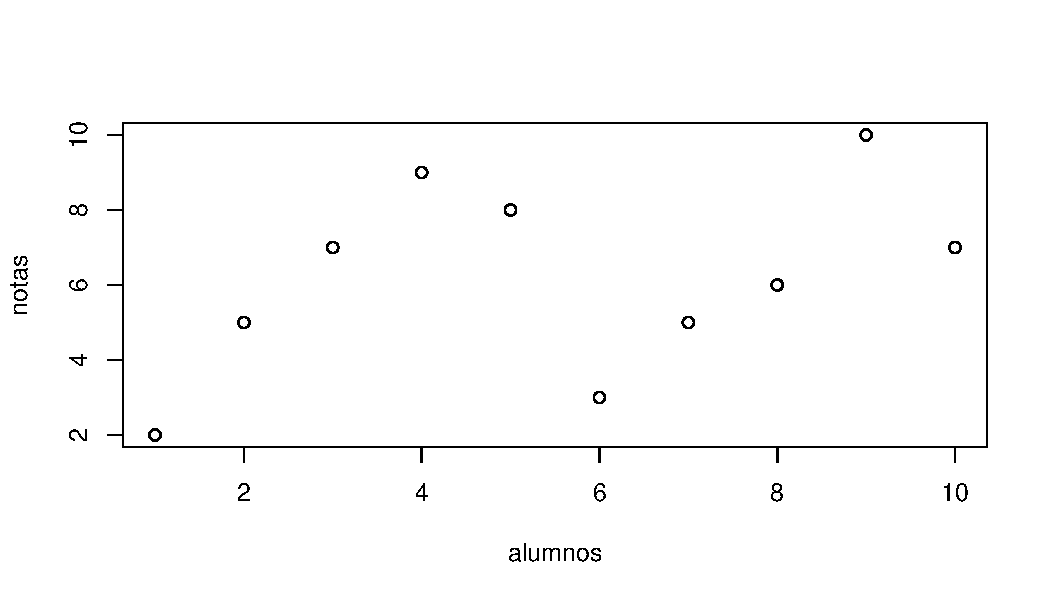
\includegraphics[width=0.75\linewidth]{Hora2_files/figure-beamer/unnamed-chunk-9-1} \end{center}
\end{frame}

\begin{frame}[fragile]{Parámetros de la función plot()}
\protect\hypertarget{paruxe1metros-de-la-funciuxf3n-plot}{}
\begin{itemize}
\tightlist
\item
  \texttt{log}: para indicar que queremos el gráfico en escala
  logarítmica
\item
  \texttt{main("título")}: para poner título al gráfico. Si en vez de un
  texto queráis poner una expresión matemática, tenéis que utilizar la
  función \texttt{expression()}
\item
  \texttt{xlab("etiqueta")}: para poner etiqueta al eje \(X\)
\item
  \texttt{ylab("etiqueta")}: para poner etiqueta al eje \(Y\)
\item
  \texttt{pch=n}: para elegir el símbolo de los puntos.
  \(n=0,1,...,25\). El valor por defecto es \texttt{pch\ =\ 1}
\item
  \texttt{cex}: para elegir el tamaño de los símbolos
\item
  \texttt{col="color\ en\ inglés"}: para elegir el color de los
  símbolos.
  \href{http://www.stat.columbia.edu/~tzheng/files/Rcolor.pdf}{Gama de
  colores}.
\end{itemize}
\end{frame}

\begin{frame}{Parámetro pch - Tipos de símbolos}
\protect\hypertarget{paruxe1metro-pch---tipos-de-suxedmbolos}{}
\begin{center}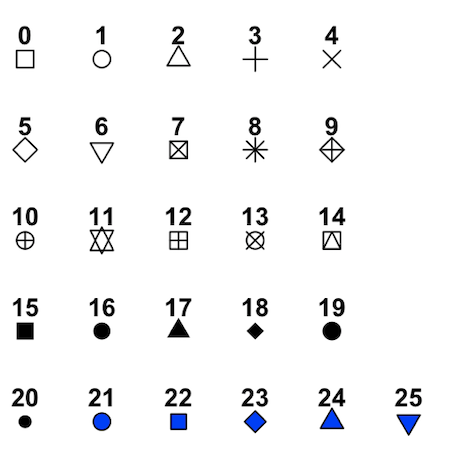
\includegraphics[width=0.6\linewidth]{Imgs/pch} \end{center}
\end{frame}

\begin{frame}[fragile]{Escala logarítmica}
\protect\hypertarget{escala-logaruxedtmica}{}
\begin{Shaded}
\begin{Highlighting}[]
\FunctionTok{par}\NormalTok{(}\AttributeTok{mfrow =} \FunctionTok{c}\NormalTok{(}\DecValTok{1}\NormalTok{,}\DecValTok{2}\NormalTok{))}
\NormalTok{plot }\OtherTok{=} \FunctionTok{plot}\NormalTok{(}\FunctionTok{exp}\NormalTok{(}\DecValTok{1}\SpecialCharTok{:}\DecValTok{20}\NormalTok{), }\AttributeTok{xlab =} \StringTok{"Indice"}\NormalTok{,}
            \AttributeTok{ylab =} \FunctionTok{expression}\NormalTok{(e}\SpecialCharTok{\^{}}\NormalTok{\{}\DecValTok{1}\SpecialCharTok{:}\DecValTok{20}\NormalTok{\}), }
            \AttributeTok{main =} \StringTok{"Escala lineal"}\NormalTok{)}
\NormalTok{plotLog }\OtherTok{=} \FunctionTok{plot}\NormalTok{(}\FunctionTok{exp}\NormalTok{(}\DecValTok{1}\SpecialCharTok{:}\DecValTok{20}\NormalTok{), }\AttributeTok{log =} \StringTok{"y"}\NormalTok{, }\AttributeTok{xlab =} \StringTok{"Indice"}\NormalTok{, }
               \AttributeTok{ylab =} \FunctionTok{expression}\NormalTok{(e}\SpecialCharTok{\^{}}\NormalTok{\{}\DecValTok{1}\SpecialCharTok{:}\DecValTok{20}\NormalTok{\}), }
               \AttributeTok{main =} \StringTok{"Escala logaritmica en el eje y"}\NormalTok{)}
\end{Highlighting}
\end{Shaded}

\begin{center}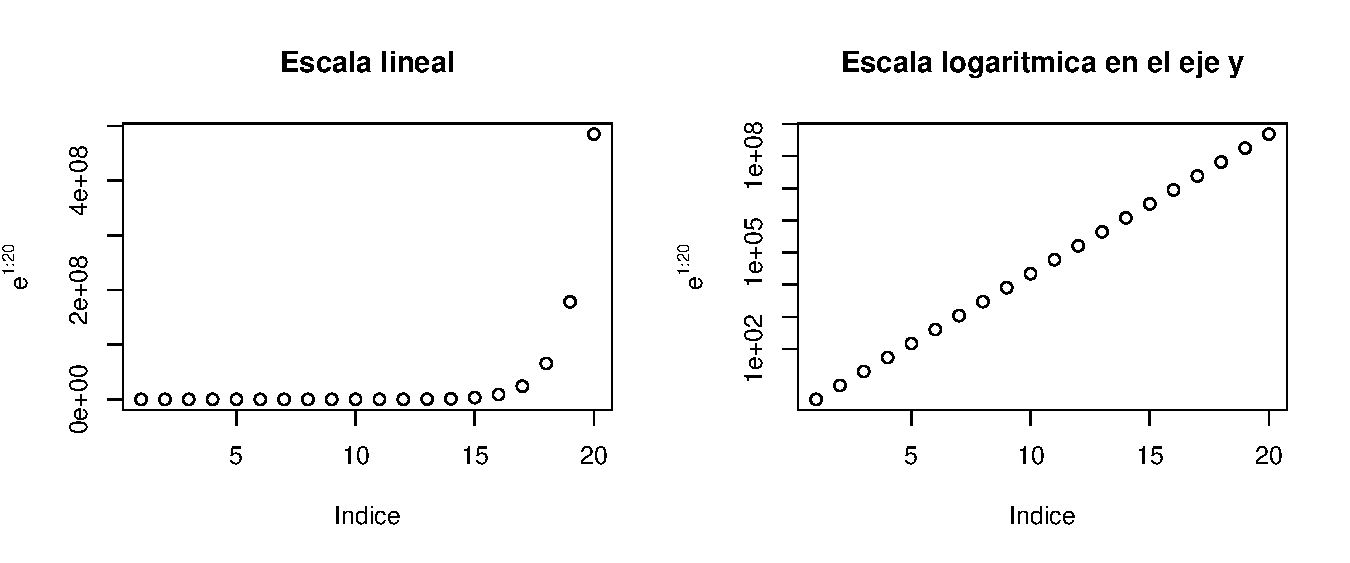
\includegraphics[width=0.7\linewidth]{Hora2_files/figure-beamer/unnamed-chunk-10-1} \end{center}

\begin{Shaded}
\begin{Highlighting}[]
\FunctionTok{par}\NormalTok{(}\AttributeTok{mfrow =} \FunctionTok{c}\NormalTok{(}\DecValTok{1}\NormalTok{,}\DecValTok{1}\NormalTok{))}
\end{Highlighting}
\end{Shaded}
\end{frame}

\begin{frame}[fragile]{Parámetros de la función plot()}
\protect\hypertarget{paruxe1metros-de-la-funciuxf3n-plot-1}{}
\begin{itemize}
\tightlist
\item
  \texttt{type}: para elegir el tipo de gráfico que queremos:

  \begin{itemize}
  \tightlist
  \item
    \texttt{p}: puntos (valor por defecto)
  \item
    \texttt{l}: líneas rectas que unen los puntos (dichos puntos no
    tienen símbolo)
  \item
    \texttt{b}: líneas rectas que unen los puntos (dichos puntos tienen
    símbolo). Las líneas no traspasan los puntos
  \item
    \texttt{o}: como el anterior pero en este caso las líneas sí que
    traspasan los puntos
  \item
    \texttt{h}: histograma de líneas
  \item
    \texttt{s}: histograma de escalones
  \item
    \texttt{n}: para no dibujar los puntos
  \end{itemize}
\end{itemize}
\end{frame}

\begin{frame}[fragile]{Tipos de gráfico}
\protect\hypertarget{tipos-de-gruxe1fico}{}
\begin{Shaded}
\begin{Highlighting}[]
\FunctionTok{par}\NormalTok{(}\AttributeTok{mfrow =} \FunctionTok{c}\NormalTok{(}\DecValTok{3}\NormalTok{,}\DecValTok{2}\NormalTok{))}
\NormalTok{x }\OtherTok{=} \FunctionTok{c}\NormalTok{(}\DecValTok{50}\SpecialCharTok{:}\DecValTok{59}\NormalTok{)}
\NormalTok{y }\OtherTok{=} \FunctionTok{c}\NormalTok{(}\DecValTok{2}\NormalTok{,}\DecValTok{9}\NormalTok{,}\DecValTok{25}\NormalTok{,}\DecValTok{3}\NormalTok{,}\DecValTok{100}\NormalTok{,}\DecValTok{77}\NormalTok{,}\DecValTok{62}\NormalTok{,}\DecValTok{54}\NormalTok{,}\DecValTok{19}\NormalTok{,}\DecValTok{40}\NormalTok{)}
\FunctionTok{plot}\NormalTok{(x,y, }\AttributeTok{pch =} \DecValTok{23}\NormalTok{, }\AttributeTok{cex =} \DecValTok{2}\NormalTok{, }\AttributeTok{col =} \StringTok{"blue"}\NormalTok{, }\AttributeTok{type =} \StringTok{"p"}\NormalTok{)}
\FunctionTok{plot}\NormalTok{(x,y, }\AttributeTok{pch =} \DecValTok{23}\NormalTok{, }\AttributeTok{cex =} \DecValTok{2}\NormalTok{, }\AttributeTok{col =} \StringTok{"blueviolet"}\NormalTok{, }\AttributeTok{type =} \StringTok{"l"}\NormalTok{)}
\FunctionTok{plot}\NormalTok{(x,y, }\AttributeTok{pch =} \DecValTok{23}\NormalTok{, }\AttributeTok{cex =} \DecValTok{2}\NormalTok{, }\AttributeTok{col =} \StringTok{"gold"}\NormalTok{, }\AttributeTok{type =} \StringTok{"b"}\NormalTok{)}
\FunctionTok{plot}\NormalTok{(x,y, }\AttributeTok{pch =} \DecValTok{23}\NormalTok{, }\AttributeTok{cex =} \DecValTok{2}\NormalTok{, }\AttributeTok{col =} \StringTok{"deeppink"}\NormalTok{, }\AttributeTok{type =} \StringTok{"o"}\NormalTok{)}
\FunctionTok{plot}\NormalTok{(x,y, }\AttributeTok{pch =} \DecValTok{23}\NormalTok{, }\AttributeTok{cex =} \DecValTok{2}\NormalTok{, }\AttributeTok{col =} \StringTok{"springgreen"}\NormalTok{,}
     \AttributeTok{type =} \StringTok{"h"}\NormalTok{)}
\FunctionTok{plot}\NormalTok{(x,y, }\AttributeTok{pch =} \DecValTok{23}\NormalTok{, }\AttributeTok{cex =} \DecValTok{2}\NormalTok{, }\AttributeTok{col =} \StringTok{"firebrick1"}\NormalTok{,}
     \AttributeTok{type =} \StringTok{"s"}\NormalTok{)}
\FunctionTok{par}\NormalTok{(}\AttributeTok{mfrow =} \FunctionTok{c}\NormalTok{(}\DecValTok{1}\NormalTok{,}\DecValTok{1}\NormalTok{))}
\end{Highlighting}
\end{Shaded}
\end{frame}

\begin{frame}{Tipos de gráfico}
\protect\hypertarget{tipos-de-gruxe1fico-1}{}
\begin{center}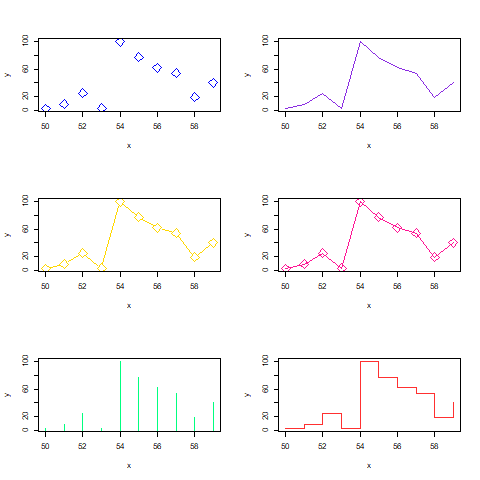
\includegraphics[width=0.7\linewidth]{Imgs/tipo_grafico_1} \end{center}
\end{frame}

\begin{frame}[fragile]{Parámetros de la función plot()}
\protect\hypertarget{paruxe1metros-de-la-funciuxf3n-plot-2}{}
\begin{itemize}
\tightlist
\item
  \texttt{lty}: para especificar el tipo de línea

  \begin{itemize}
  \tightlist
  \item
    ``solid'' : \(1\): línea continua (valor por defecto)
  \item
    ``dashed'' : \(2\): línea discontinua
  \item
    ``dotted'' : \(3\): línea de puntos
  \item
    ``dotdashed'' : \(4\): línea que alterna puntos y rayas
  \end{itemize}
\item
  \texttt{lwd}: para especificar el grosor de las líneas
\item
  \texttt{xlim}: para modificar el rango del eje \(X\)
\item
  \texttt{ylim}: para modificar el rango del eje \(Y\)
\item
  \texttt{xaxp}: para modificar posiciones de las marcas en el eje \(X\)
\item
  \texttt{yaxp}: para modificar posiciones de las marcas en el eje \(Y\)
\end{itemize}
\end{frame}

\begin{frame}[fragile]{Parámetros de la función plot()}
\protect\hypertarget{paruxe1metros-de-la-funciuxf3n-plot-3}{}
\begin{Shaded}
\begin{Highlighting}[]
\NormalTok{x }\OtherTok{=}\NormalTok{ (}\DecValTok{2}\SpecialCharTok{*}\NormalTok{(}\DecValTok{1}\SpecialCharTok{:}\DecValTok{20}\NormalTok{))}
\NormalTok{y }\OtherTok{=}\NormalTok{ (}\SpecialCharTok{{-}}\DecValTok{1}\NormalTok{)}\SpecialCharTok{\^{}}\NormalTok{(}\DecValTok{1}\SpecialCharTok{:}\DecValTok{20}\NormalTok{)}\SpecialCharTok{*}\DecValTok{5}\SpecialCharTok{*}\NormalTok{(}\DecValTok{1}\SpecialCharTok{:}\DecValTok{20}\NormalTok{)}
\FunctionTok{plot}\NormalTok{(x,y, }\AttributeTok{main =} \StringTok{"Ejemplo de grafico"}\NormalTok{, }\AttributeTok{pch =} \DecValTok{8}\NormalTok{, }\AttributeTok{cex =} \DecValTok{1}\NormalTok{,}
     \AttributeTok{type =} \StringTok{"b"}\NormalTok{, }\AttributeTok{lty =} \DecValTok{4}\NormalTok{, }\AttributeTok{lwd =} \DecValTok{4}\NormalTok{, }
     \AttributeTok{xaxp =} \FunctionTok{c}\NormalTok{(}\DecValTok{0}\NormalTok{,}\DecValTok{40}\NormalTok{,}\DecValTok{2}\NormalTok{), }\AttributeTok{yaxp =} \FunctionTok{c}\NormalTok{(}\SpecialCharTok{{-}}\DecValTok{100}\NormalTok{,}\DecValTok{100}\NormalTok{,}\DecValTok{8}\NormalTok{))}
\end{Highlighting}
\end{Shaded}

\begin{center}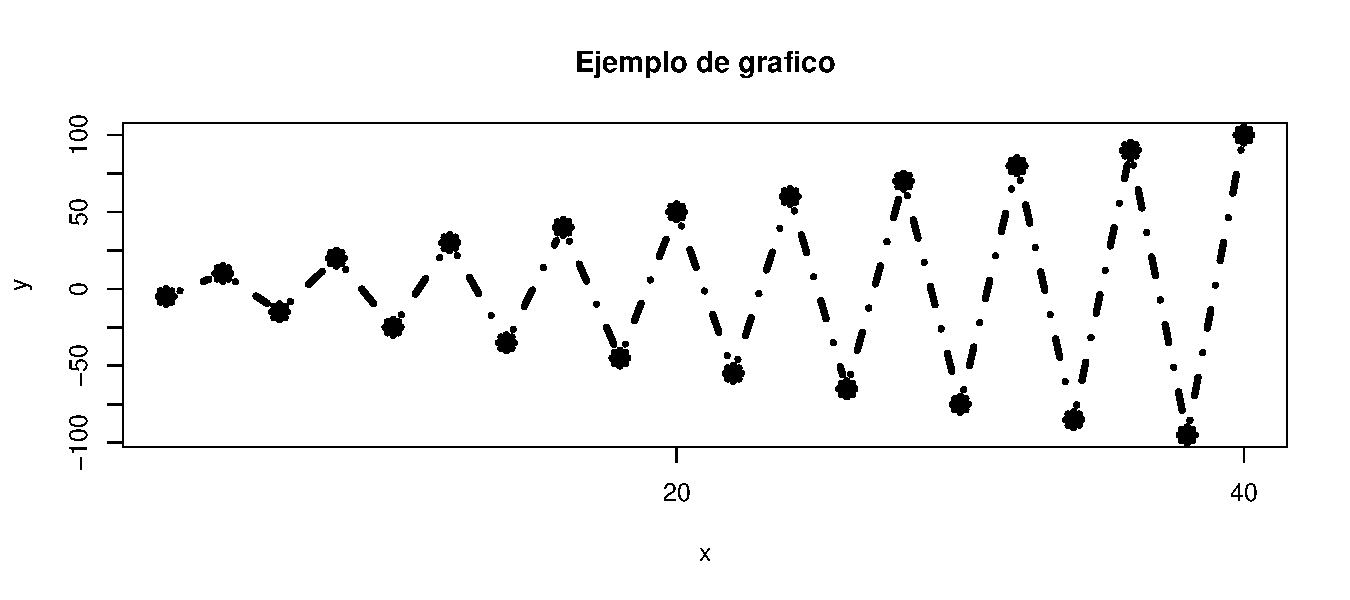
\includegraphics[width=0.8\linewidth]{Hora2_files/figure-beamer/unnamed-chunk-12-1} \end{center}
\end{frame}

\begin{frame}[fragile]{Añadir elementos al gráfico}
\protect\hypertarget{auxf1adir-elementos-al-gruxe1fico}{}
\begin{itemize}
\tightlist
\item
  \texttt{points(x,y)}: añade un punto de coordenadas \((x, y)\) a un
  gráfico ya existente
\item
  \texttt{abline}: para añadir una recta a un gráfico ya existente

  \begin{itemize}
  \tightlist
  \item
    \texttt{abline(a,b)}: añade la recta \(y=ax+b\)
  \item
    \texttt{abline(v\ =\ x0)}: añade la recta vertical \(x=x_0\). \(v\)
    puede estar asignado a un vector
  \item
    \texttt{abline(h\ =\ y0)}: añade la recta horizontal \(y=y_0\).
    \(h\) puede estar asignado a un vector
  \end{itemize}
\end{itemize}
\end{frame}

\begin{frame}[fragile]{Añadiendo punto y recta}
\protect\hypertarget{auxf1adiendo-punto-y-recta}{}
\begin{Shaded}
\begin{Highlighting}[]
\NormalTok{x }\OtherTok{=}\NormalTok{ (}\DecValTok{2}\SpecialCharTok{*}\NormalTok{(}\DecValTok{1}\SpecialCharTok{:}\DecValTok{20}\NormalTok{))}
\NormalTok{y }\OtherTok{=}\NormalTok{ (}\SpecialCharTok{{-}}\DecValTok{1}\NormalTok{)}\SpecialCharTok{\^{}}\NormalTok{(}\DecValTok{1}\SpecialCharTok{:}\DecValTok{20}\NormalTok{)}\SpecialCharTok{*}\DecValTok{5}\SpecialCharTok{*}\NormalTok{(}\DecValTok{1}\SpecialCharTok{:}\DecValTok{20}\NormalTok{)}
\FunctionTok{plot}\NormalTok{(x,y, }\AttributeTok{main =} \StringTok{"Poniendo un punto y una recta"}\NormalTok{, }\AttributeTok{pch =} \DecValTok{8}\NormalTok{,}
     \AttributeTok{cex =} \DecValTok{1}\NormalTok{, }\AttributeTok{type =} \StringTok{"b"}\NormalTok{, }\AttributeTok{lty =} \DecValTok{4}\NormalTok{, }
     \AttributeTok{lwd =} \DecValTok{4}\NormalTok{, }\AttributeTok{xaxp =} \FunctionTok{c}\NormalTok{(}\DecValTok{0}\NormalTok{,}\DecValTok{40}\NormalTok{,}\DecValTok{2}\NormalTok{), }\AttributeTok{yaxp =} \FunctionTok{c}\NormalTok{(}\SpecialCharTok{{-}}\DecValTok{100}\NormalTok{,}\DecValTok{100}\NormalTok{,}\DecValTok{8}\NormalTok{))}
\FunctionTok{points}\NormalTok{(}\DecValTok{20}\NormalTok{,}\DecValTok{0}\NormalTok{, }\AttributeTok{col =} \StringTok{"red"}\NormalTok{, }\AttributeTok{cex =} \DecValTok{4}\NormalTok{, }\AttributeTok{pch =} \DecValTok{16}\NormalTok{)}
\FunctionTok{abline}\NormalTok{ (}\AttributeTok{h =} \DecValTok{0}\NormalTok{, }\AttributeTok{lty =} \DecValTok{2}\NormalTok{, }\AttributeTok{col =} \StringTok{"dodgerblue"}\NormalTok{)}
\end{Highlighting}
\end{Shaded}
\end{frame}

\begin{frame}{Añadiendo punto y recta}
\protect\hypertarget{auxf1adiendo-punto-y-recta-1}{}
\begin{center}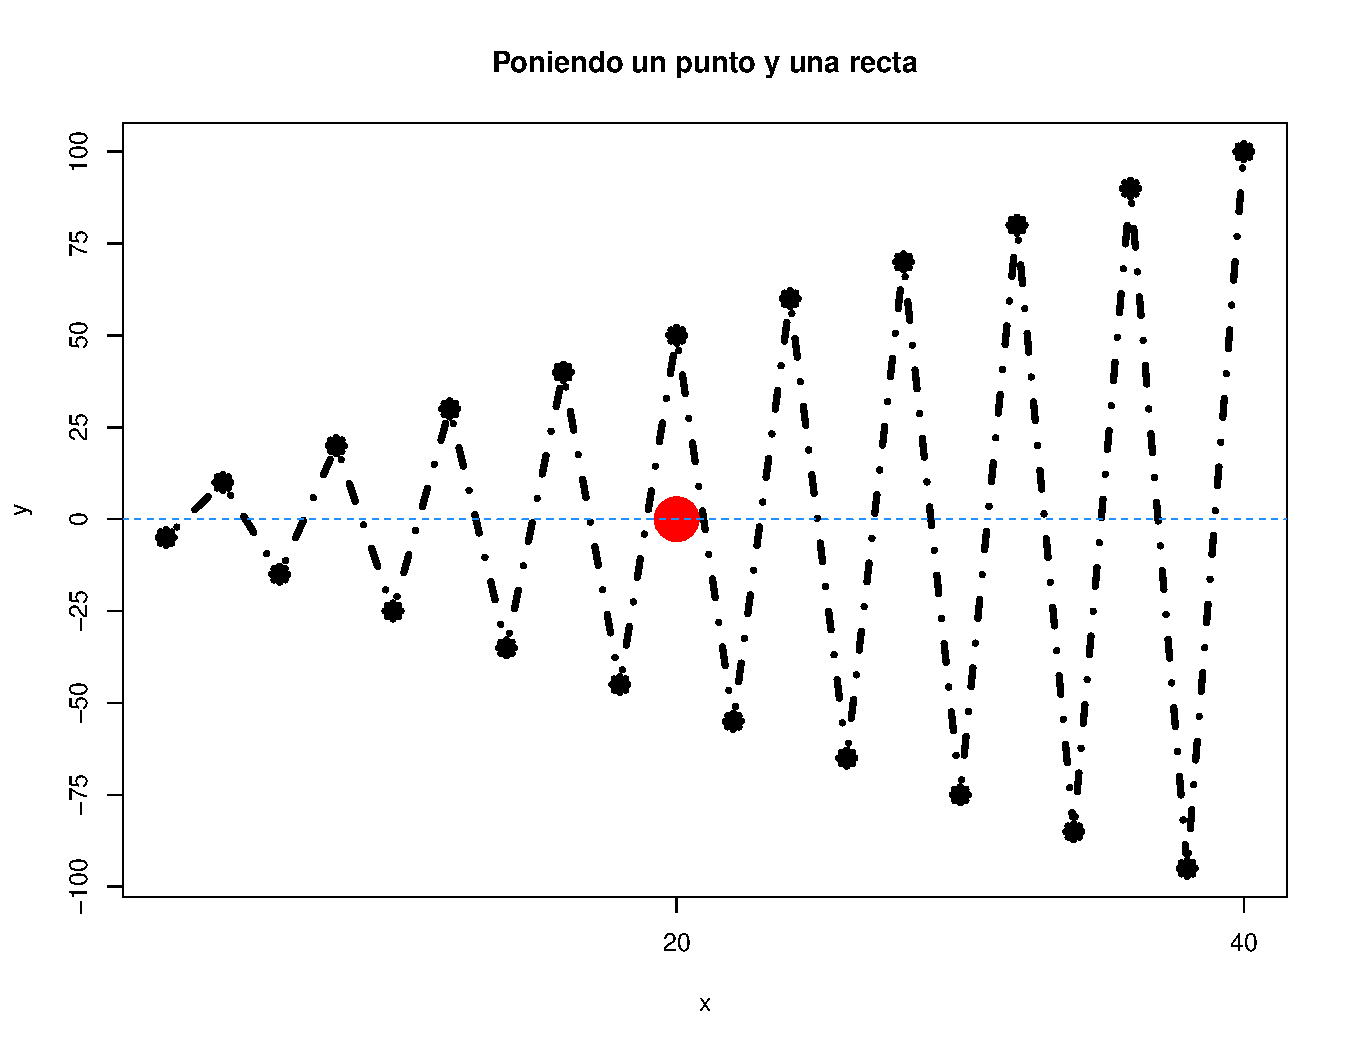
\includegraphics[width=0.65\linewidth]{Hora2_files/figure-beamer/unnamed-chunk-14-1} \end{center}
\end{frame}

\begin{frame}[fragile]{Añadir elementos al gráfico}
\protect\hypertarget{auxf1adir-elementos-al-gruxe1fico-1}{}
\begin{itemize}
\tightlist
\item
  \texttt{text(x,y,labels\ =\ "....")}: añade en el punto de coordenadas
  \((x,y)\) el texto especificado como argumento de labels

  \begin{itemize}
  \tightlist
  \item
    \texttt{pos}: permite indicar la posición del texto alrededor de las
    coordenadas \((x,y)\). Admite los siguientes valores:

    \begin{itemize}
    \tightlist
    \item
      1: abajo
    \item
      2: izquierda
    \item
      3: arriba
    \item
      4: derecha
    \item
      5: sin especificar: el texto se sitúa centrado en el punto
      \((x,y)\)
    \end{itemize}
  \end{itemize}
\end{itemize}
\end{frame}

\begin{frame}[fragile]{Añadiendo etiquetas}
\protect\hypertarget{auxf1adiendo-etiquetas}{}
\begin{Shaded}
\begin{Highlighting}[]
\NormalTok{alumnos }\OtherTok{=} \FunctionTok{c}\NormalTok{(}\DecValTok{1}\SpecialCharTok{:}\DecValTok{10}\NormalTok{)}
\NormalTok{notas }\OtherTok{=} \FunctionTok{c}\NormalTok{(}\DecValTok{2}\NormalTok{,}\DecValTok{5}\NormalTok{,}\DecValTok{7}\NormalTok{,}\DecValTok{9}\NormalTok{,}\DecValTok{8}\NormalTok{,}\DecValTok{3}\NormalTok{,}\DecValTok{5}\NormalTok{,}\DecValTok{6}\NormalTok{,}\DecValTok{10}\NormalTok{,}\DecValTok{7}\NormalTok{)}
\FunctionTok{plot}\NormalTok{(alumnos,notas, }\AttributeTok{main =} \StringTok{"Grafico con texto"}\NormalTok{)}
\FunctionTok{text}\NormalTok{(alumnos,notas, }
     \AttributeTok{labels =} \FunctionTok{c}\NormalTok{(}\StringTok{"S"}\NormalTok{,}\StringTok{"A"}\NormalTok{,}\StringTok{"N"}\NormalTok{,}\StringTok{"E"}\NormalTok{,}\StringTok{"N"}\NormalTok{,}\StringTok{"S"}\NormalTok{,}\StringTok{"A"}\NormalTok{,}\StringTok{"A"}\NormalTok{,}\StringTok{"E"}\NormalTok{,}\StringTok{"N"}\NormalTok{), }
     \AttributeTok{pos =} \FunctionTok{c}\NormalTok{(}\FunctionTok{rep}\NormalTok{(}\DecValTok{3}\NormalTok{,}\AttributeTok{times =} \DecValTok{8}\NormalTok{),}\DecValTok{1}\NormalTok{,}\DecValTok{3}\NormalTok{))}
\end{Highlighting}
\end{Shaded}

\begin{center}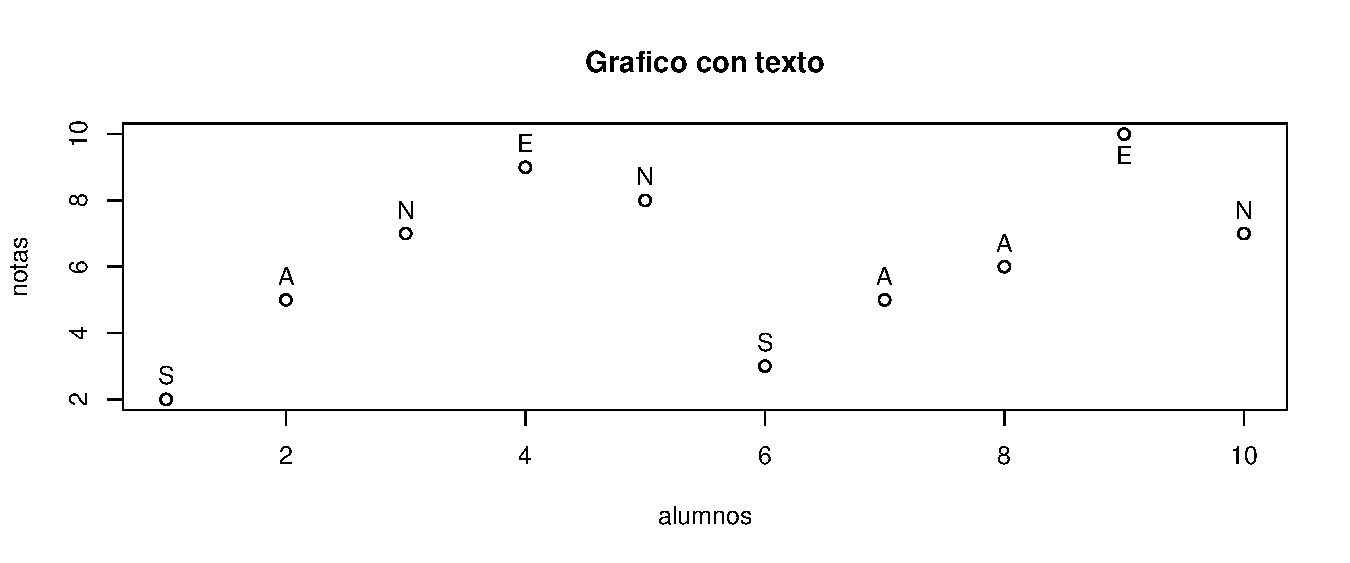
\includegraphics[width=0.8\linewidth]{Hora2_files/figure-beamer/unnamed-chunk-15-1} \end{center}
\end{frame}

\begin{frame}[fragile]{Añadir elementos al gráfico}
\protect\hypertarget{auxf1adir-elementos-al-gruxe1fico-2}{}
\begin{itemize}
\tightlist
\item
  \texttt{lines(x,\ y)}:añade a un gráfico existente una línea poligonal
  que une los puntos \((x_i, y_i)\) sucesivos. \(x,y\) son vectores
  numéricos
\item
  \texttt{curve(curva)}: permite añadir la gráfica de una curva a un
  gráfico existente

  \begin{itemize}
  \tightlist
  \item
    \texttt{add=TRUE}: si no, la curva no se añade
  \item
    La curva se puede especificar mediante una expresión algebraica con
    variable \(x\), o mediante su nombre si la hemos definido antes
  \end{itemize}
\end{itemize}
\end{frame}

\begin{frame}[fragile]{Añadiendo líneas y curvas}
\protect\hypertarget{auxf1adiendo-luxedneas-y-curvas}{}
\begin{Shaded}
\begin{Highlighting}[]
\NormalTok{x }\OtherTok{=} \FunctionTok{c}\NormalTok{(}\DecValTok{5}\SpecialCharTok{*}\NormalTok{(}\DecValTok{1}\SpecialCharTok{:}\DecValTok{20}\NormalTok{))}
\FunctionTok{plot}\NormalTok{(x,}\FunctionTok{c}\NormalTok{(}\FunctionTok{exp}\NormalTok{(}\SpecialCharTok{{-}}\NormalTok{x)}\SpecialCharTok{+}\NormalTok{(}\SpecialCharTok{{-}}\DecValTok{1}\NormalTok{)}\SpecialCharTok{\^{}}\NormalTok{x}\SpecialCharTok{*}\NormalTok{x}\SpecialCharTok{/}\DecValTok{2}\SpecialCharTok{*}\FunctionTok{sin}\NormalTok{(x)}\SpecialCharTok{\^{}}\DecValTok{2}\NormalTok{))}
\FunctionTok{lines}\NormalTok{(}\FunctionTok{c}\NormalTok{(}\DecValTok{20}\NormalTok{,}\DecValTok{10}\NormalTok{,}\DecValTok{40}\NormalTok{,}\DecValTok{80}\NormalTok{,}\DecValTok{60}\NormalTok{,}\DecValTok{60}\NormalTok{,}\DecValTok{20}\NormalTok{),}\FunctionTok{c}\NormalTok{(}\DecValTok{20}\NormalTok{,}\DecValTok{0}\NormalTok{,}\SpecialCharTok{{-}}\DecValTok{20}\NormalTok{,}\SpecialCharTok{{-}}\DecValTok{20}\NormalTok{,}\DecValTok{40}\NormalTok{,}\DecValTok{0}\NormalTok{,}\DecValTok{20}\NormalTok{), }
      \AttributeTok{lwd =} \DecValTok{2}\NormalTok{, }\AttributeTok{col =} \StringTok{"darkslategray1"}\NormalTok{)}
\FunctionTok{curve}\NormalTok{(}\DecValTok{20}\SpecialCharTok{*}\FunctionTok{sin}\NormalTok{(x), }\AttributeTok{add =} \ConstantTok{TRUE}\NormalTok{, }\AttributeTok{col =} \StringTok{"green"}\NormalTok{)}
\end{Highlighting}
\end{Shaded}

\begin{center}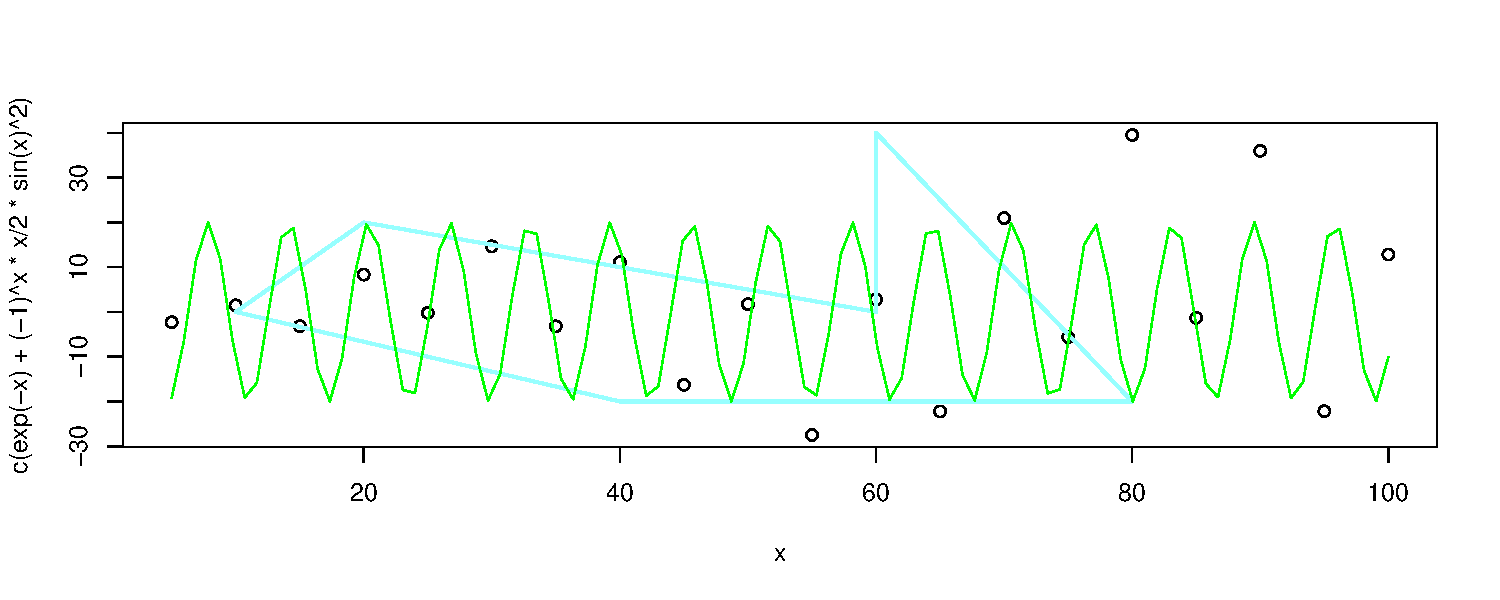
\includegraphics[width=0.8\linewidth]{Hora2_files/figure-beamer/unnamed-chunk-16-1} \end{center}
\end{frame}

\begin{frame}[fragile]{Añadir elementos al gráfico}
\protect\hypertarget{auxf1adir-elementos-al-gruxe1fico-3}{}
\begin{itemize}
\tightlist
\item
  \texttt{legend(posición,\ legend\ =\ ...)}: para añadir una leyenda

  \begin{itemize}
  \tightlist
  \item
    La posición indica donde queremos situar la leyenda. Puede ser o
    bien las coordenadas de la esquina superior izquierda de nuestra
    leyenda, o bien una de las palabras siguientes:

    \begin{itemize}
    \tightlist
    \item
      ``bottom'' / ``bottomright'' / ``bottomleft''
    \item
      ``top'' / ``topright'' / ``topleft''
    \item
      ``center'' / ``right'' / ``left''
    \end{itemize}
  \item
    \texttt{legend}: contiene el vector de nombres entre comillas con
    los que queremos identificar a las curvas en la leyenda
  \end{itemize}
\end{itemize}
\end{frame}

\begin{frame}[fragile]{Añadiendo leyenda}
\protect\hypertarget{auxf1adiendo-leyenda}{}
\begin{Shaded}
\begin{Highlighting}[]
\NormalTok{x }\OtherTok{=} \FunctionTok{seq}\NormalTok{(}\DecValTok{0}\NormalTok{,}\DecValTok{2}\SpecialCharTok{*}\NormalTok{pi,}\FloatTok{0.1}\NormalTok{)}
\FunctionTok{plot}\NormalTok{(x,}\FunctionTok{sin}\NormalTok{(x),}\AttributeTok{type=}\StringTok{"l"}\NormalTok{,}\AttributeTok{col=}\StringTok{"blue"}\NormalTok{,}\AttributeTok{lwd=}\DecValTok{3}\NormalTok{, }\AttributeTok{xlab=}\StringTok{""}\NormalTok{, }\AttributeTok{ylab=}\StringTok{""}\NormalTok{)}
\FunctionTok{lines}\NormalTok{(x,}\FunctionTok{cos}\NormalTok{(x),}\AttributeTok{col=}\StringTok{"green"}\NormalTok{,}\AttributeTok{lwd=}\DecValTok{3}\NormalTok{)}
\FunctionTok{lines}\NormalTok{(x, }\FunctionTok{tan}\NormalTok{(x), }\AttributeTok{col=}\StringTok{"purple"}\NormalTok{,}\AttributeTok{lwd=}\DecValTok{3}\NormalTok{)}
\FunctionTok{legend}\NormalTok{(}\StringTok{"bottomleft"}\NormalTok{,}\AttributeTok{col=}\FunctionTok{c}\NormalTok{(}\StringTok{"blue"}\NormalTok{,}\StringTok{"green"}\NormalTok{,}\StringTok{"purple"}\NormalTok{), }
       \AttributeTok{legend=}\FunctionTok{c}\NormalTok{(}\StringTok{"Seno"}\NormalTok{,}\StringTok{"Coseno"}\NormalTok{, }\StringTok{"Tangente"}\NormalTok{), }
       \AttributeTok{lwd=}\DecValTok{3}\NormalTok{, }\AttributeTok{bty=}\StringTok{"l"}\NormalTok{)}
\end{Highlighting}
\end{Shaded}
\end{frame}

\begin{frame}{Añadiendo leyenda}
\protect\hypertarget{auxf1adiendo-leyenda-1}{}
\begin{center}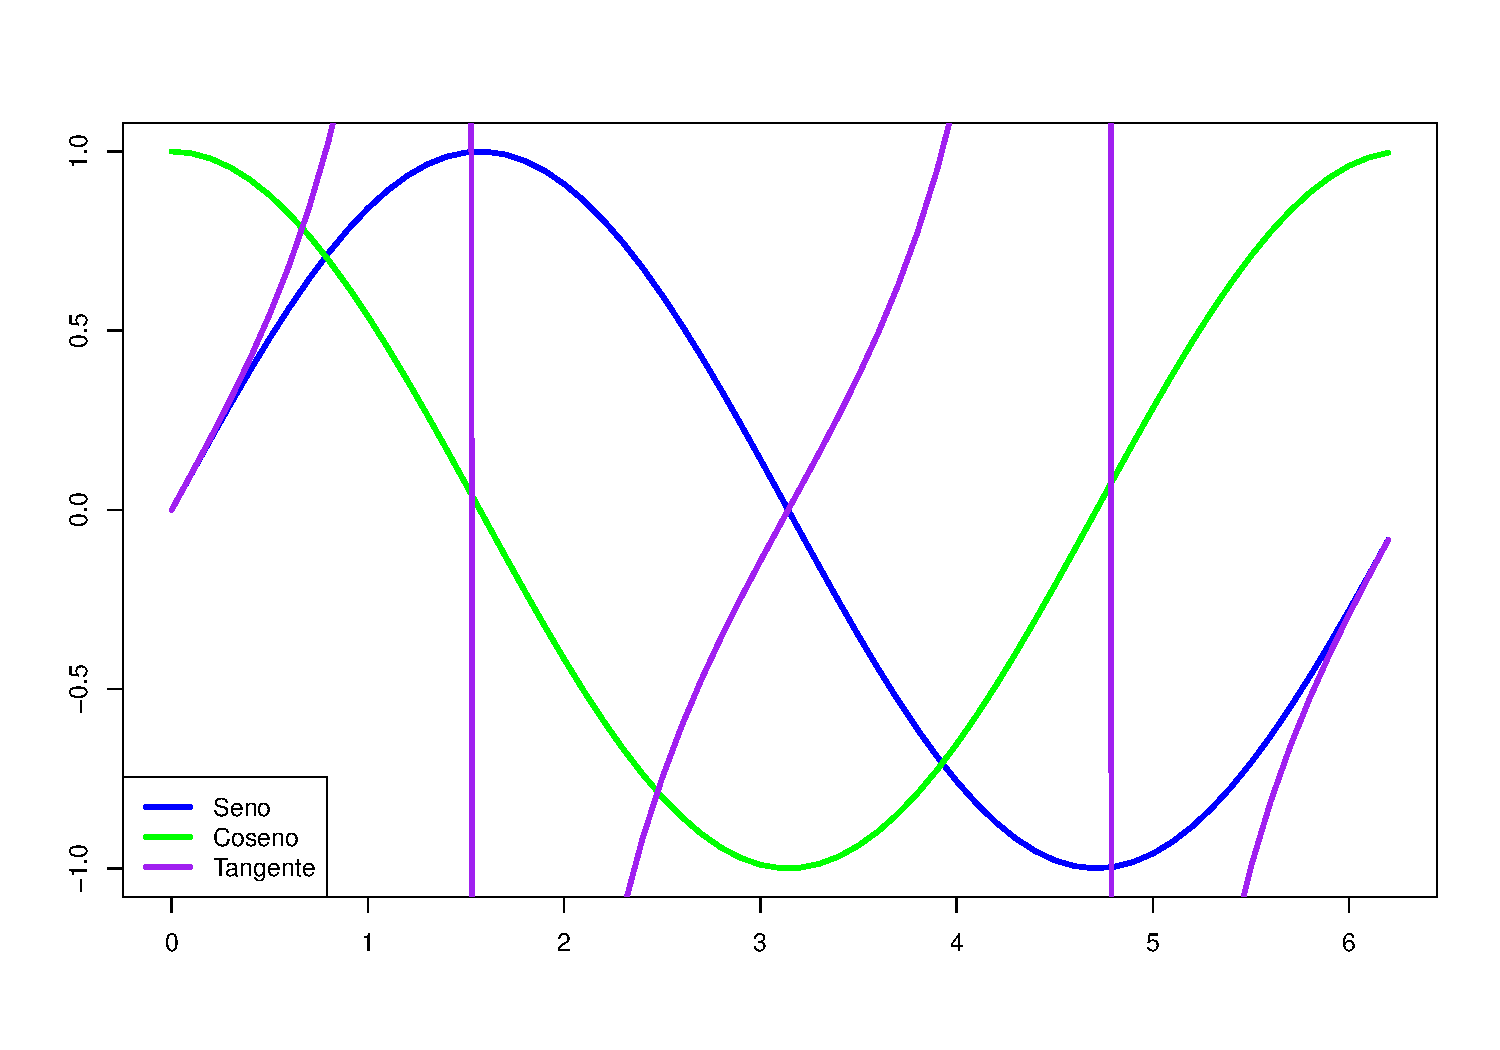
\includegraphics[width=0.75\linewidth]{Hora2_files/figure-beamer/unnamed-chunk-18-1} \end{center}
\end{frame}

\begin{frame}[fragile]{Añadir elementos al gráfico}
\protect\hypertarget{auxf1adir-elementos-al-gruxe1fico-4}{}
\begin{itemize}
\tightlist
\item
  \texttt{segments}: para añadir segmentos a un gráfico existente
\item
  \texttt{arrows}: para añadir flechas a un gráfico existente
\item
  \texttt{symbols}: para añadir símbolos a un gráfico existente
\item
  \texttt{polygon}: para añadir polígonos cerrados especificando sus
  vértices a un gráfico existente
\end{itemize}
\end{frame}

\begin{frame}[fragile]{Añadiendo elementos}
\protect\hypertarget{auxf1adiendo-elementos}{}
\begin{Shaded}
\begin{Highlighting}[]
\NormalTok{x }\OtherTok{=} \FunctionTok{c}\NormalTok{(}\DecValTok{5}\SpecialCharTok{*}\NormalTok{(}\DecValTok{1}\SpecialCharTok{:}\DecValTok{10}\NormalTok{))}
\FunctionTok{plot}\NormalTok{(x,}\FunctionTok{c}\NormalTok{(}\FunctionTok{exp}\NormalTok{(}\SpecialCharTok{{-}}\NormalTok{x)}\SpecialCharTok{+}\NormalTok{(}\SpecialCharTok{{-}}\DecValTok{1}\NormalTok{)}\SpecialCharTok{\^{}}\NormalTok{x}\SpecialCharTok{*}\NormalTok{x}\SpecialCharTok{/}\DecValTok{2}\SpecialCharTok{*}\FunctionTok{sin}\NormalTok{(x)}\SpecialCharTok{\^{}}\DecValTok{2}\NormalTok{), }\AttributeTok{xlab =} \StringTok{""}\NormalTok{, }\AttributeTok{ylab =} \StringTok{""}\NormalTok{, }
     \AttributeTok{main =} \StringTok{"Grafico con varios elementos"}\NormalTok{)}
\FunctionTok{segments}\NormalTok{(}\DecValTok{10}\NormalTok{,}\DecValTok{0}\NormalTok{,}\DecValTok{40}\NormalTok{,}\DecValTok{0}\NormalTok{, }\AttributeTok{col =} \StringTok{"red"}\NormalTok{, }\AttributeTok{lwd =} \DecValTok{4}\NormalTok{)}
\FunctionTok{arrows}\NormalTok{(}\DecValTok{10}\NormalTok{,}\DecValTok{0}\NormalTok{,}\DecValTok{40}\NormalTok{,}\SpecialCharTok{{-}}\DecValTok{10}\NormalTok{, }\AttributeTok{col =} \StringTok{" blue"}\NormalTok{, }\AttributeTok{length =} \FloatTok{0.5}\NormalTok{,}
       \AttributeTok{angle =} \DecValTok{5}\NormalTok{, }\AttributeTok{code =} \DecValTok{3}\NormalTok{)}
\FunctionTok{symbols}\NormalTok{(}\DecValTok{40}\NormalTok{,}\DecValTok{0}\NormalTok{,}\AttributeTok{stars =} \FunctionTok{cbind}\NormalTok{(}\DecValTok{1}\NormalTok{,.}\DecValTok{5}\NormalTok{,}\DecValTok{1}\NormalTok{,.}\DecValTok{5}\NormalTok{,}\DecValTok{1}\NormalTok{,.}\DecValTok{5}\NormalTok{,}\DecValTok{1}\NormalTok{,.}\DecValTok{5}\NormalTok{,}\DecValTok{1}\NormalTok{,.}\DecValTok{5}\NormalTok{), }
        \AttributeTok{add =} \ConstantTok{TRUE}\NormalTok{, }\AttributeTok{lwd =} \DecValTok{3}\NormalTok{, }\AttributeTok{inches =} \FloatTok{0.5}\NormalTok{)}
\FunctionTok{symbols}\NormalTok{(}\DecValTok{40}\NormalTok{,}\DecValTok{0}\NormalTok{,}\AttributeTok{stars =} \FunctionTok{cbind}\NormalTok{(}\DecValTok{1}\NormalTok{,.}\DecValTok{5}\NormalTok{,}\DecValTok{1}\NormalTok{,.}\DecValTok{5}\NormalTok{,}\DecValTok{1}\NormalTok{,.}\DecValTok{5}\NormalTok{,}\DecValTok{1}\NormalTok{,.}\DecValTok{5}\NormalTok{,}\DecValTok{1}\NormalTok{,.}\DecValTok{5}\NormalTok{),}
        \AttributeTok{add =} \ConstantTok{TRUE}\NormalTok{, }\AttributeTok{lwd =} \DecValTok{3}\NormalTok{)}
\FunctionTok{polygon}\NormalTok{(}\FunctionTok{c}\NormalTok{(}\DecValTok{20}\NormalTok{,}\DecValTok{30}\NormalTok{,}\DecValTok{40}\NormalTok{),}\FunctionTok{c}\NormalTok{(}\DecValTok{10}\NormalTok{,}\SpecialCharTok{{-}}\DecValTok{10}\NormalTok{,}\DecValTok{10}\NormalTok{), }\AttributeTok{col =} \StringTok{"gold"}\NormalTok{,}
        \AttributeTok{density =} \DecValTok{3}\NormalTok{, }\AttributeTok{angle =} \DecValTok{90}\NormalTok{, }\AttributeTok{lty =} \DecValTok{4}\NormalTok{, }
        \AttributeTok{lwd =} \DecValTok{5}\NormalTok{)}
\end{Highlighting}
\end{Shaded}
\end{frame}

\begin{frame}{Añadiendo elementos}
\protect\hypertarget{auxf1adiendo-elementos-1}{}
\begin{center}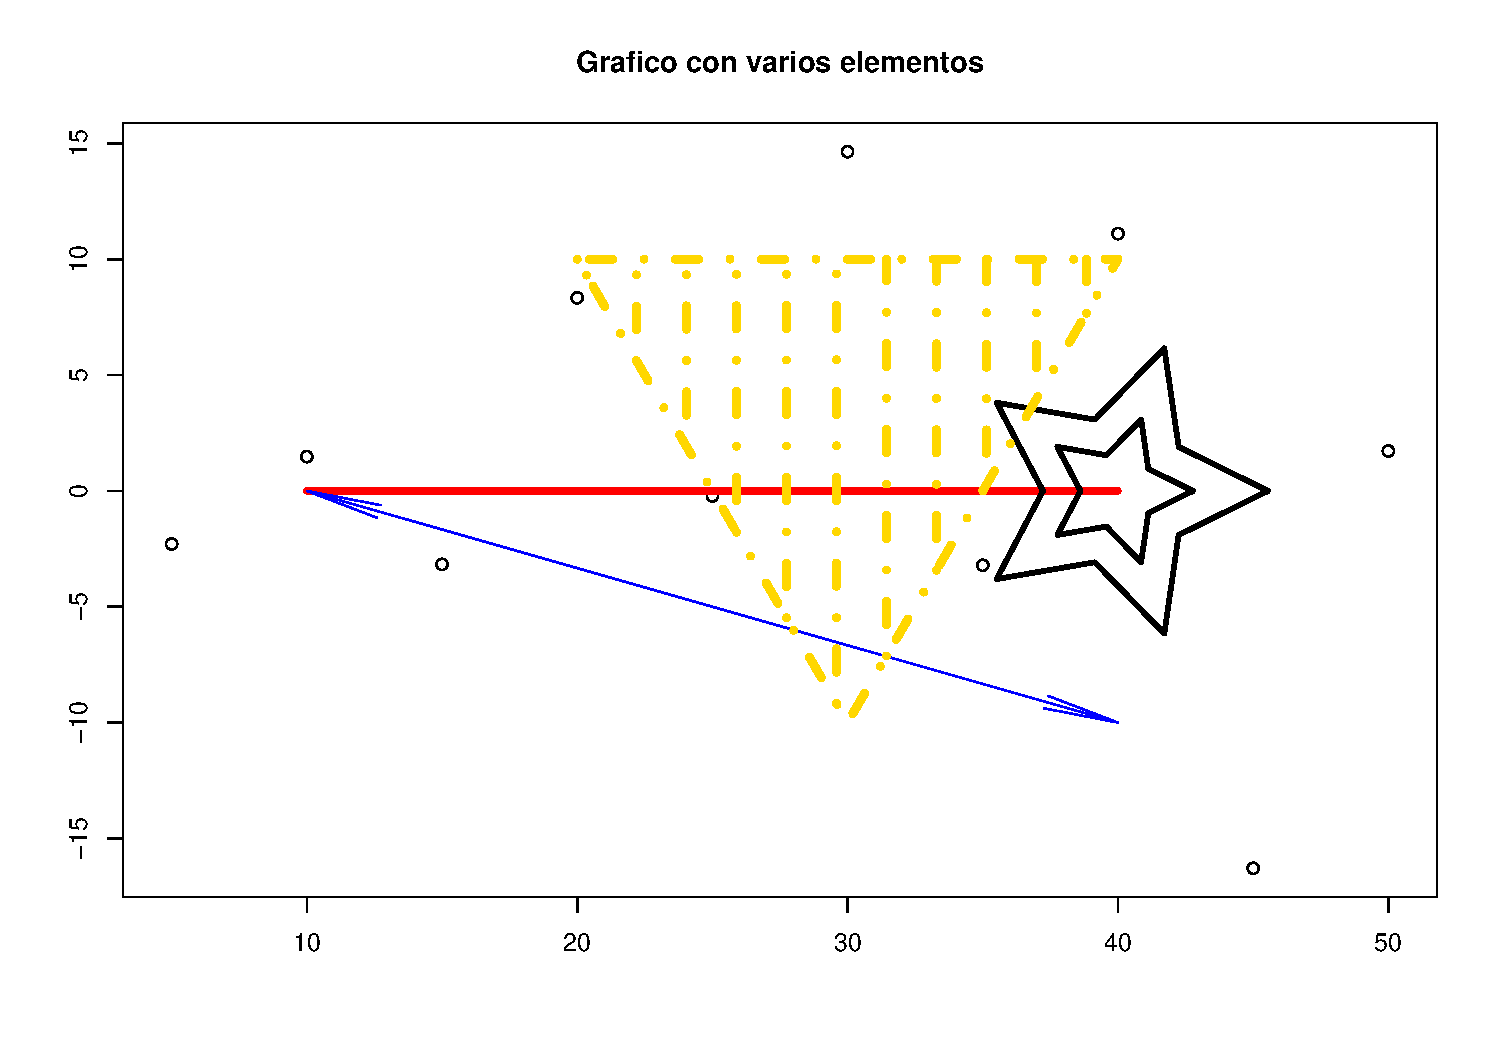
\includegraphics[width=0.75\linewidth]{Hora2_files/figure-beamer/unnamed-chunk-20-1} \end{center}
\end{frame}

\hypertarget{hojas-de-datos-data-frames}{%
\section{Hojas de datos: data frames}\label{hojas-de-datos-data-frames}}

\begin{frame}[fragile]{Data frames}
\protect\hypertarget{data-frames}{}
\blue{Data frame.} Un data frame es una tabla de doble entrada, formada
por variables en las columnas y observaciones de estas variables en las
filas, de manera que cada fila contiene los valores de las variables
para un mismo caso o un mismo individuo.

\begin{itemize}
\item
  \texttt{data()}: para abrir una ventana con la lista de los objetos de
  datos a los que tenemos acceso en la sesión actual de R (los que lleva
  la instalación básica de R y los que aportan los paquetes que tengamos
  cargados.

  \begin{itemize}
  \tightlist
  \item
    Si entramos \texttt{data(package=.packages(all.available\ =\ TRUE))}
    obtendremos la lista de todos los objetos de datos a los que tenemos
    acceso, incluyendo los de los paquetes que tengamos instalados, pero
    que no estén cargados en la sesión actual.
  \end{itemize}
\end{itemize}
\end{frame}

\begin{frame}[fragile]{Acceder a la información, estructura y atributos
de un data frame}
\protect\hypertarget{acceder-a-la-informaciuxf3n-estructura-y-atributos-de-un-data-frame}{}
\begin{itemize}
\tightlist
\item
  \texttt{head(d.f,n)}: para mostrar las \(n\) primeras filas del data
  frame. Por defecto se muestran las 6 primeras filas
\item
  \texttt{tail(d.f,n)}: para mostrar las \(n\) últimas filas del data
  frame. Por defecto semuestran las 6 últimas
\item
  \texttt{str(d.f)}: para conocer la estructura global de un data frame
\item
  \texttt{names(d.f)}: para producir un vector con los nombres de las
  columnas
\end{itemize}
\end{frame}

\begin{frame}[fragile]{Acceder a la información, estructura y atributos
de un data frame}
\protect\hypertarget{acceder-a-la-informaciuxf3n-estructura-y-atributos-de-un-data-frame-1}{}
\begin{Shaded}
\begin{Highlighting}[]
\FunctionTok{str}\NormalTok{(Orange)}
\end{Highlighting}
\end{Shaded}

\begin{verbatim}
Classes 'nfnGroupedData', 'nfGroupedData', 'groupedData' and 'data.frame':  35 obs. of  3 variables:
 $ Tree         : Ord.factor w/ 5 levels "3"<"1"<"5"<"2"<..: 2 2 2 2 2 2 2 4 4 4 ...
 $ age          : num  118 484 664 1004 1231 ...
 $ circumference: num  30 58 87 115 120 142 145 33 69 111 ...
 - attr(*, "formula")=Class 'formula'  language circumference ~ age | Tree
  .. ..- attr(*, ".Environment")=<environment: R_EmptyEnv> 
 - attr(*, "labels")=List of 2
  ..$ x: chr "Time since December 31, 1968"
  ..$ y: chr "Trunk circumference"
 - attr(*, "units")=List of 2
  ..$ x: chr "(days)"
  ..$ y: chr "(mm)"
\end{verbatim}
\end{frame}

\begin{frame}[fragile]{Acceder a la información, estructura y atributos
de un data frame}
\protect\hypertarget{acceder-a-la-informaciuxf3n-estructura-y-atributos-de-un-data-frame-2}{}
\begin{Shaded}
\begin{Highlighting}[]
\FunctionTok{head}\NormalTok{(Orange,}\DecValTok{4}\NormalTok{)}
\end{Highlighting}
\end{Shaded}

\begin{verbatim}
  Tree  age circumference
1    1  118            30
2    1  484            58
3    1  664            87
4    1 1004           115
\end{verbatim}

\begin{Shaded}
\begin{Highlighting}[]
\FunctionTok{tail}\NormalTok{(Orange,}\DecValTok{4}\NormalTok{)}
\end{Highlighting}
\end{Shaded}

\begin{verbatim}
   Tree  age circumference
32    5 1004           125
33    5 1231           142
34    5 1372           174
35    5 1582           177
\end{verbatim}
\end{frame}

\begin{frame}[fragile]{Acceder a la información, estructura y atributos
de un data frame}
\protect\hypertarget{acceder-a-la-informaciuxf3n-estructura-y-atributos-de-un-data-frame-3}{}
\begin{itemize}
\tightlist
\item
  \texttt{rownames(d.f)}: para producir un vector con los
  identificadores de las filas

  \begin{itemize}
  \tightlist
  \item
    R entiende siempre que estos identificadores son palabras, aunque
    sean números, de ahí que los imprima entre comillas
  \end{itemize}
\item
  \texttt{colnames(d.f)}: para producir un vector con los
  identificadores de las columnas
\item
  \texttt{dimnames(d.f)}: para producir una list formada por dos
  vectores (el de los identificadores de las filas y el de los nombres
  de las columnas)
\item
  \texttt{nrow(d.f)}: para consultar el número de filas de un data frame
\item
  \texttt{ncol(d.f)}: para consultar el número de columnas de un data
  frame
\item
  \texttt{dim(d.f)}: para producir un vector con el número de filas y el
  de columnas
\end{itemize}
\end{frame}

\begin{frame}[fragile]{Acceder a la información, estructura y atributos
de un data frame}
\protect\hypertarget{acceder-a-la-informaciuxf3n-estructura-y-atributos-de-un-data-frame-4}{}
\begin{itemize}
\tightlist
\item
  \texttt{d.f\$nombre\_variable}: para obtener una columna concreta de
  un dataframe

  \begin{itemize}
  \tightlist
  \item
    El resultado será un vector o un factor, según cómo esté definida la
    columna dentro del data frame
  \item
    Las variables de un data frame son internas, no están definidas en
    el entorno global de trabajo de R
  \end{itemize}
\end{itemize}
\end{frame}

\begin{frame}[fragile]{Sub-data frames}
\protect\hypertarget{sub-data-frames}{}
\begin{itemize}
\tightlist
\item
  \texttt{d.f{[}n,m{]}}: para extraer ``trozos'' del data frame por
  filas y columnas (funciona exactamente igual que en matrices) donde
  \(n\) y \(m\) pueden definirse como:

  \begin{itemize}
  \tightlist
  \item
    intervalos
  \item
    condiciones
  \item
    números naturales
  \item
    no poner nada
  \item
    Si sólo queremos definir la subtabla quedándonos con algunas
    variables, basta aplicar el nombre del data frame al vector de
    variables
  \item
    Estas construcciones se pueden usar también para reordenar las filas
    o columnas
  \end{itemize}
\end{itemize}
\end{frame}

\begin{frame}[fragile]{Sub-data frames}
\protect\hypertarget{sub-data-frames-1}{}
\begin{Shaded}
\begin{Highlighting}[]
\NormalTok{dataOrange }\OtherTok{=}\NormalTok{ Orange}
\NormalTok{dataOrange[}\FunctionTok{c}\NormalTok{(}\DecValTok{10}\SpecialCharTok{:}\DecValTok{12}\NormalTok{),]}
\end{Highlighting}
\end{Shaded}

\begin{verbatim}
   Tree  age circumference
10    2  664           111
11    2 1004           156
12    2 1231           172
\end{verbatim}

\begin{Shaded}
\begin{Highlighting}[]
\NormalTok{dataOrange[}\FunctionTok{c}\NormalTok{(}\DecValTok{2}\NormalTok{,}\DecValTok{17}\NormalTok{),}\FunctionTok{c}\NormalTok{(}\DecValTok{1}\NormalTok{,}\DecValTok{3}\NormalTok{)]}
\end{Highlighting}
\end{Shaded}

\begin{verbatim}
   Tree circumference
2     1            58
17    3            75
\end{verbatim}
\end{frame}

\begin{frame}[fragile]{Sub-data frames}
\protect\hypertarget{sub-data-frames-2}{}
\begin{Shaded}
\begin{Highlighting}[]
\NormalTok{dataOrange[}\DecValTok{2}\NormalTok{,}\DecValTok{3}\NormalTok{]}
\end{Highlighting}
\end{Shaded}

\begin{verbatim}
[1] 58
\end{verbatim}

\begin{Shaded}
\begin{Highlighting}[]
\NormalTok{dataOrange[dataOrange}\SpecialCharTok{$}\NormalTok{circumference}\SpecialCharTok{\textless{}=}\DecValTok{50}\NormalTok{,]}
\end{Highlighting}
\end{Shaded}

\begin{verbatim}
   Tree age circumference
1     1 118            30
8     2 118            33
15    3 118            30
22    4 118            32
29    5 118            30
30    5 484            49
\end{verbatim}
\end{frame}

\begin{frame}[fragile]{Leyendo tablas de datos}
\protect\hypertarget{leyendo-tablas-de-datos}{}
\begin{itemize}
\tightlist
\item
  \texttt{read.table()}: para definir un data frame a partir de una
  tabla de datos contenida en un fichero

  \begin{itemize}
  \tightlist
  \item
    Este fichero puede estar guardado en nuestro ordenador o bien
    podemos conocer su url. Sea cual sea el caso, se aplica la función
    al nombre del fichero o a la dirección entre comillas
  \end{itemize}
\end{itemize}

Aquí tenéis una \href{http://aprender.uib.es/}{lista de data frames}
para practicar
\end{frame}

\begin{frame}[fragile]{Parámetros de la función read.table()}
\protect\hypertarget{paruxe1metros-de-la-funciuxf3n-read.table}{}
\begin{itemize}
\tightlist
\item
  \texttt{header\ =\ TRUE}: para indicar si la tabla que importamos
  tiene una primera fila con los nombres de las columnas. El valor por
  defecto es FALSE
\item
  \texttt{col.names\ =\ c(...)}: para especificar el nombre de las
  columnas. No olvidéis que cada nombre debe ir entre comillas
\item
  \texttt{sep}: para especificar las separaciones entre columnas en el
  fichero (si no es un espacio en blanco). Si es así, hay que introducir
  el parámetro pertinente entre comillas
\item
  \texttt{dec}: para especificar el signo que separa la parte entera de
  la decimal (si no es un punto. Si es así, hay que introducir el
  parámetro pertinente entre comillas
\end{itemize}
\end{frame}

\begin{frame}[fragile]{Parámetros de read.table()}
\protect\hypertarget{paruxe1metros-de-read.table}{}
\begin{Shaded}
\begin{Highlighting}[]
\NormalTok{notas }\OtherTok{=} \FunctionTok{read.table}\NormalTok{(}
  \StringTok{"http://aprender.uib.es/Rdir/Controls11{-}12.txt"}\NormalTok{, }
  \AttributeTok{col.names =} \FunctionTok{c}\NormalTok{(}\StringTok{"Nota\_Parcial"}\NormalTok{,}\StringTok{"Nota\_Final"}\NormalTok{,}\StringTok{"Grup"}\NormalTok{),}
  \AttributeTok{sep=}\StringTok{","}\NormalTok{,}\AttributeTok{header=}\ConstantTok{TRUE}\NormalTok{)}
\FunctionTok{head}\NormalTok{(notas,}\DecValTok{8}\NormalTok{)}
\end{Highlighting}
\end{Shaded}

\begin{verbatim}
  Nota_Parcial Nota_Final Grup
1           35         34    1
2           45         30    0
3           64         19    1
4           67         30    0
5           82         31    0
6           50         34    1
7           68         30    0
8           46         23    2
\end{verbatim}
\end{frame}

\begin{frame}[fragile]{Más parámetros de read.table()}
\protect\hypertarget{muxe1s-paruxe1metros-de-read.table}{}
\begin{itemize}
\item
  \texttt{stringsAsFactors}: para prohibir la transformación de las
  columnas de palabras en factores debemos usar
  \texttt{stringsAsFactors=FALSE} (ya que por defecto, R realiza dicha
  transformación)
\item
  Para importar un fichero de una página web segura (cuyo url empiece
  con https), no podemos entrar directamente la dirección en
  \texttt{read.table()}; una solución es instalar y cargar el paquete
  RCurl y entonces usar la instrucción
  \texttt{read.table\ (textConnection(getURL(“url\ ”)),...)}.
\end{itemize}
\end{frame}

\begin{frame}[fragile]{Otros formatos de fichero de datos}
\protect\hypertarget{otros-formatos-de-fichero-de-datos}{}
\begin{itemize}
\tightlist
\item
  \texttt{read.csv()}: para importar ficheros en formato CSV
\item
  \texttt{read.xls()} o \texttt{read.xlsx()}: para importar hojas de
  cálculo tipo Excel u OpenOffice en formato XLS o XLSX,
  respectivamente. Se necesita el paquete xlsx
\item
  \texttt{read.mtb()}: para importar tablas de datos Minitab. Se
  necesita el paquete foreign
\item
  \texttt{read.spss()}: para importar tablas de datos SPSS. Se necesita
  el paquete foreign
\end{itemize}
\end{frame}

\begin{frame}[fragile]{Exportación de datos a ficheros}
\protect\hypertarget{exportaciuxf3n-de-datos-a-ficheros}{}
\begin{itemize}
\tightlist
\item
  \texttt{write.table(df,\ file\ =\ "")}: para exportar un data frame a
  un fichero

  \begin{itemize}
  \tightlist
  \item
    \texttt{file\ =\ ""}: es donde indicaremos el nombre que queremos
    darle al fichero
  \item
    Podemos usar el parámetro \texttt{sep} para indicar el símbolo de
    separación de columnas. Siempre entre comillas
  \item
    También podemos utilizar el parámetro \texttt{dec} para indicar la
    separación entre la parte entera y decimal de los datos
  \end{itemize}
\end{itemize}
\end{frame}

\begin{frame}[fragile]{Exportando datos a ficheros}
\protect\hypertarget{exportando-datos-a-ficheros}{}
\begin{Shaded}
\begin{Highlighting}[]
\FunctionTok{write.table}\NormalTok{(notas, }\AttributeTok{file =} \StringTok{"../data/NotasData.csv"}\NormalTok{,}
            \AttributeTok{dec =} \StringTok{"."}\NormalTok{)}
\NormalTok{notas2 }\OtherTok{=} \FunctionTok{read.table}\NormalTok{(}\StringTok{"../data/NotasData.csv"}\NormalTok{, }\AttributeTok{header =} \ConstantTok{TRUE}\NormalTok{)}
\FunctionTok{str}\NormalTok{(notas2)}
\end{Highlighting}
\end{Shaded}

\begin{verbatim}
'data.frame':   156 obs. of  3 variables:
 $ Nota_Parcial: int  35 45 64 67 82 50 68 46 43 77 ...
 $ Nota_Final  : int  34 30 19 30 31 34 30 23 51 53 ...
 $ Grup        : int  1 0 1 0 0 1 0 2 2 1 ...
\end{verbatim}
\end{frame}

\begin{frame}[fragile]{Crear data frames}
\protect\hypertarget{crear-data-frames}{}
\begin{itemize}
\tightlist
\item
  \texttt{data.frame(vector\_1,...,vector\_n)}: para construir un data
  frame a partir de vectores introducidos en el orden en el que queremos
  disponer las columnas de la tabla

  \begin{itemize}
  \tightlist
  \item
    R considera del mismo tipo de datos todas las entradas de una
    columna de un data frame
  \item
    Las variables tomarán los nombres de los vectores. Estos nombres se
    pueden especificar en el argumento de \texttt{data.frame} entrando
    una construcción de la forma \texttt{nombre\_variable\ =\ vector}
  \item
    \texttt{rownames}: para especificar los identificadores de las filas
  \item
    También en esta función podemos hacer uso del parámetro
    \texttt{stringsAsFactors} para evitar la transformación de las
    columnas de tipo palabra en factores
  \end{itemize}
\end{itemize}
\end{frame}

\begin{frame}[fragile]{Crear data frames}
\protect\hypertarget{crear-data-frames-1}{}
\begin{Shaded}
\begin{Highlighting}[]
\NormalTok{Programacion }\OtherTok{=} \FunctionTok{c}\NormalTok{(}\DecValTok{1}\NormalTok{,}\DecValTok{2}\NormalTok{,}\DecValTok{0}\NormalTok{,}\DecValTok{5}\NormalTok{,}\DecValTok{4}\NormalTok{,}\DecValTok{6}\NormalTok{,}\DecValTok{7}\NormalTok{,}\DecValTok{5}\NormalTok{,}\DecValTok{5}\NormalTok{,}\DecValTok{8}\NormalTok{)}
\NormalTok{Calculo }\OtherTok{=} \FunctionTok{c}\NormalTok{(}\DecValTok{3}\NormalTok{,}\DecValTok{3}\NormalTok{,}\DecValTok{2}\NormalTok{,}\DecValTok{7}\NormalTok{,}\DecValTok{9}\NormalTok{,}\DecValTok{5}\NormalTok{,}\DecValTok{6}\NormalTok{,}\DecValTok{8}\NormalTok{,}\DecValTok{5}\NormalTok{,}\DecValTok{6}\NormalTok{)}
\NormalTok{Empresa }\OtherTok{=} \FunctionTok{c}\NormalTok{(}\DecValTok{4}\NormalTok{,}\DecValTok{5}\NormalTok{,}\DecValTok{4}\NormalTok{,}\DecValTok{8}\NormalTok{,}\DecValTok{8}\NormalTok{,}\DecValTok{9}\NormalTok{,}\DecValTok{6}\NormalTok{,}\DecValTok{7}\NormalTok{,}\DecValTok{9}\NormalTok{,}\DecValTok{10}\NormalTok{)}
\NormalTok{grados }\OtherTok{=} \FunctionTok{data.frame}\NormalTok{(}\AttributeTok{Pr =}\NormalTok{ Programacion, }
                    \AttributeTok{Ca =}\NormalTok{ Calculo, }\AttributeTok{Em =}\NormalTok{ Empresa)}
\FunctionTok{str}\NormalTok{(grados)}
\end{Highlighting}
\end{Shaded}

\begin{verbatim}
'data.frame':   10 obs. of  3 variables:
 $ Pr: num  1 2 0 5 4 6 7 5 5 8
 $ Ca: num  3 3 2 7 9 5 6 8 5 6
 $ Em: num  4 5 4 8 8 9 6 7 9 10
\end{verbatim}
\end{frame}

\begin{frame}[fragile]{Crear data frames}
\protect\hypertarget{crear-data-frames-2}{}
\begin{itemize}
\tightlist
\item
  \texttt{fix(d.f)}: para crear / editar un data frame con el editor de
  datos
\item
  \texttt{names(d.f)}: para cambiar los nombres de las variables
\item
  \texttt{rownames(d.f)}: para modificar los identificadores de las
  filas. Han de ser todos diferentes
\item
  \texttt{dimnames(d.f)=list(vec\_nom\_fil,\ vec\_nom\_col)}: para
  modificar el nombre de las filas y de las columnas simultáneamente
\end{itemize}
\end{frame}

\begin{frame}[fragile]{Crear data frames}
\protect\hypertarget{crear-data-frames-3}{}
\begin{itemize}
\tightlist
\item
  \texttt{d.f{[}núm\_fila,{]}\ =\ c(...)}: para añadir una fila a un
  data frame

  \begin{itemize}
  \tightlist
  \item
    Las filas que añadimos de esta manera son vectores, y por tanto sus
    entradas han de ser todas del mismo tipo
  \item
    Si no añadimos las filas inmediatamente siguientes a la última fila
    del data frame, los valores entre su última fila y las que añadimos
    quedarán no definidos y aparecerán como NA
  \item
    Para evitar el problema anterior, vale más usar la función
    \texttt{rbind()} para concatenar el data frame con la nueva fila
  \end{itemize}
\end{itemize}
\end{frame}

\begin{frame}[fragile]{Crear data frames}
\protect\hypertarget{crear-data-frames-4}{}
\begin{Shaded}
\begin{Highlighting}[]
\NormalTok{Ingles }\OtherTok{=} \FunctionTok{c}\NormalTok{(}\DecValTok{5}\NormalTok{,}\DecValTok{4}\NormalTok{,}\DecValTok{6}\NormalTok{,}\DecValTok{2}\NormalTok{,}\DecValTok{1}\NormalTok{,}\DecValTok{0}\NormalTok{,}\DecValTok{7}\NormalTok{,}\DecValTok{8}\NormalTok{,}\DecValTok{9}\NormalTok{,}\DecValTok{6}\NormalTok{)}
\NormalTok{grados2 }\OtherTok{=} \FunctionTok{cbind}\NormalTok{(grados, Ingles)}
\FunctionTok{head}\NormalTok{(grados2)}
\end{Highlighting}
\end{Shaded}

\begin{verbatim}
  Pr Ca Em Ingles
1  1  3  4      5
2  2  3  5      4
3  0  2  4      6
4  5  7  8      2
5  4  9  8      1
6  6  5  9      0
\end{verbatim}
\end{frame}

\begin{frame}[fragile]{Crear data frames}
\protect\hypertarget{crear-data-frames-5}{}
\begin{itemize}
\tightlist
\item
  \texttt{d.f\$new\_var}: para añadir una nueva variable al data frame

  \begin{itemize}
  \tightlist
  \item
    Podemos concatenar columnas con un data frame existente mediante la
    función \texttt{cbind()}. De este modo se puede añadir la columna
    directamente sin necesidad de convertirla antes a data frame
  \item
    Esta nueva variable ha de tener la misma longitud que el resto de
    columnas del data frame original. Si no, se añadirán valores NA a
    las variables del data frame original o a la nueva variable hasta
    completar la misma longitud
  \end{itemize}
\end{itemize}
\end{frame}

\begin{frame}[fragile]{Cambiando los tipos de datos}
\protect\hypertarget{cambiando-los-tipos-de-datos}{}
\begin{itemize}
\tightlist
\item
  \texttt{as.character}: para transformar todos los datos de un objeto
  en palabras
\item
  \texttt{as.integer}: para transformar todos los datos de un objeto a
  números enteros
\item
  \texttt{as.numeric}: para transformar todos los datos de un objeto a
  números reales
\end{itemize}
\end{frame}

\begin{frame}[fragile]{Más sobre sub-data frames}
\protect\hypertarget{muxe1s-sobre-sub-data-frames}{}
\begin{itemize}
\item
  \texttt{droplevels(d.f)}: para borrar los niveles sobrantes de todos
  los factores, ya que las columnas que son factores heredan en los
  sub-data frames todos los niveles del factor original, aunque no
  aparezcan en el trozo que hemos extraído
\item
  \texttt{select(d.f,\ parámetros)}: para especificar que queremos
  extraer de un data frame

  \begin{itemize}
  \tightlist
  \item
    \texttt{starts\_with("x")}: extrae del data frame las variables cuyo
    nombre empieza con la palabra ``x''
  \item
    \texttt{ends\_with("x")}: extrae del data frame las variables cuyo
    nombre termina con la palabra ``x''
  \item
    \texttt{contains("x")}: extrae del data frame las variables cuyo
    nombre contiene la palabra ``x''
  \item
    Se necesita el paquete \texttt{dplyr} o mejor aún \texttt{tidyverse}
  \end{itemize}
\end{itemize}
\end{frame}

\begin{frame}[fragile]{Más sobre sub-data frames}
\protect\hypertarget{muxe1s-sobre-sub-data-frames-1}{}
\begin{itemize}
\tightlist
\item
  \texttt{subset(d.f,condición,select\ =\ columnas)}: para extraer del
  data frame las filas que cumplen la condición y las columnas
  especificadas

  \begin{itemize}
  \tightlist
  \item
    Si queremos todas las filas, no hay que especificar ninguna
    condición
  \item
    Si queremos todas las columnas, no hace especificar el parámetro
    \texttt{select}
  \item
    Las variables en la condición se especifican con su nombre, sin
    añadir antes el nombre del data frame
  \end{itemize}
\end{itemize}
\end{frame}

\begin{frame}[fragile]{Aplicando funciones a data frames}
\protect\hypertarget{aplicando-funciones-a-data-frames}{}
\begin{itemize}
\tightlist
\item
  \texttt{sapply(d.f,\ función)}: para aplicar una función a todas las
  columnas de un data frame en un solo paso

  \begin{itemize}
  \tightlist
  \item
    \texttt{na.rm=TRUE}: para evitar que el valor que devuelva la
    función para las columnas que contengan algún NA sea NA
  \end{itemize}
\item
  \texttt{aggregate(variables\textasciitilde{}factors,data=d.f,FUN=función)}:
  para aplicar una función a variables de un data frame clasificadas por
  los niveles de un, o más de un, factor

  \begin{itemize}
  \tightlist
  \item
    Si queremos aplicar la función a más de una variable, tenemos que
    agruparlas con un \texttt{cbind}
  \item
    Si queremos separar las variables mediante más de un factor, tenemos
    que agruparlos con signos \(+\)
  \end{itemize}
\end{itemize}
\end{frame}

\begin{frame}[fragile]{Variables globales}
\protect\hypertarget{variables-globales}{}
No son funciones de \red{R etiqueta}

\begin{itemize}
\tightlist
\item
  \texttt{attach(d.f)}: para hacer que R entienda sus variables como
  globales y que las podamos usar por su nombre, sin necesidad de añadir
  delante el nombre del data frame y el símbolo \$

  \begin{itemize}
  \tightlist
  \item
    Si ya hubiera existido una variable definida con el mismo nombre que
    una variable del data frame al que aplicamos \texttt{attach},
    hubiéramos obtenido un mensaje de error al ejecutar esta función y
    no se hubiera reescrito la variable global original
  \end{itemize}
\item
  \texttt{detach(d.f)}: para devolver la situación original, eliminando
  del entorno global las variables del data frame
\end{itemize}
\end{frame}

\end{document}
